\chapter{CMS Detector and Reconstruction}

\section{Introduction}

The LHC is a $27\unit{km}$ circular particle accelerator which lies across the
French-Swiss border about $100\unit{m}$ underground. It was designed to accelerate and 
collide beams of protons or heavy ions. The design centre of mass energy
($\sqrt{s}$) for proton-proton collisions is $14\unit{TeV}$. The design 
luminosity is $10^{34}\unit{cm^{-2}s^{-1}}$. The LHC is the highest energy 
particle accelerator ever built. \\

Figure \ref{fig:LHC} shows a diagram of the LHC accelerator complex. Protons are
extracted from a cylinder of hydrogen gas and accelerated first by a linear
accelerator which injects them into the Proton Synchrotron (PS), which 
accelerates them to $25\unit{GeV}$ and feeds the Super Proton Synchrotron 
(SPS). The SPS accelerates the beams to $450\unit{GeV}$ and subsequently injects 
them into the LHC. \\

\begin{figure}
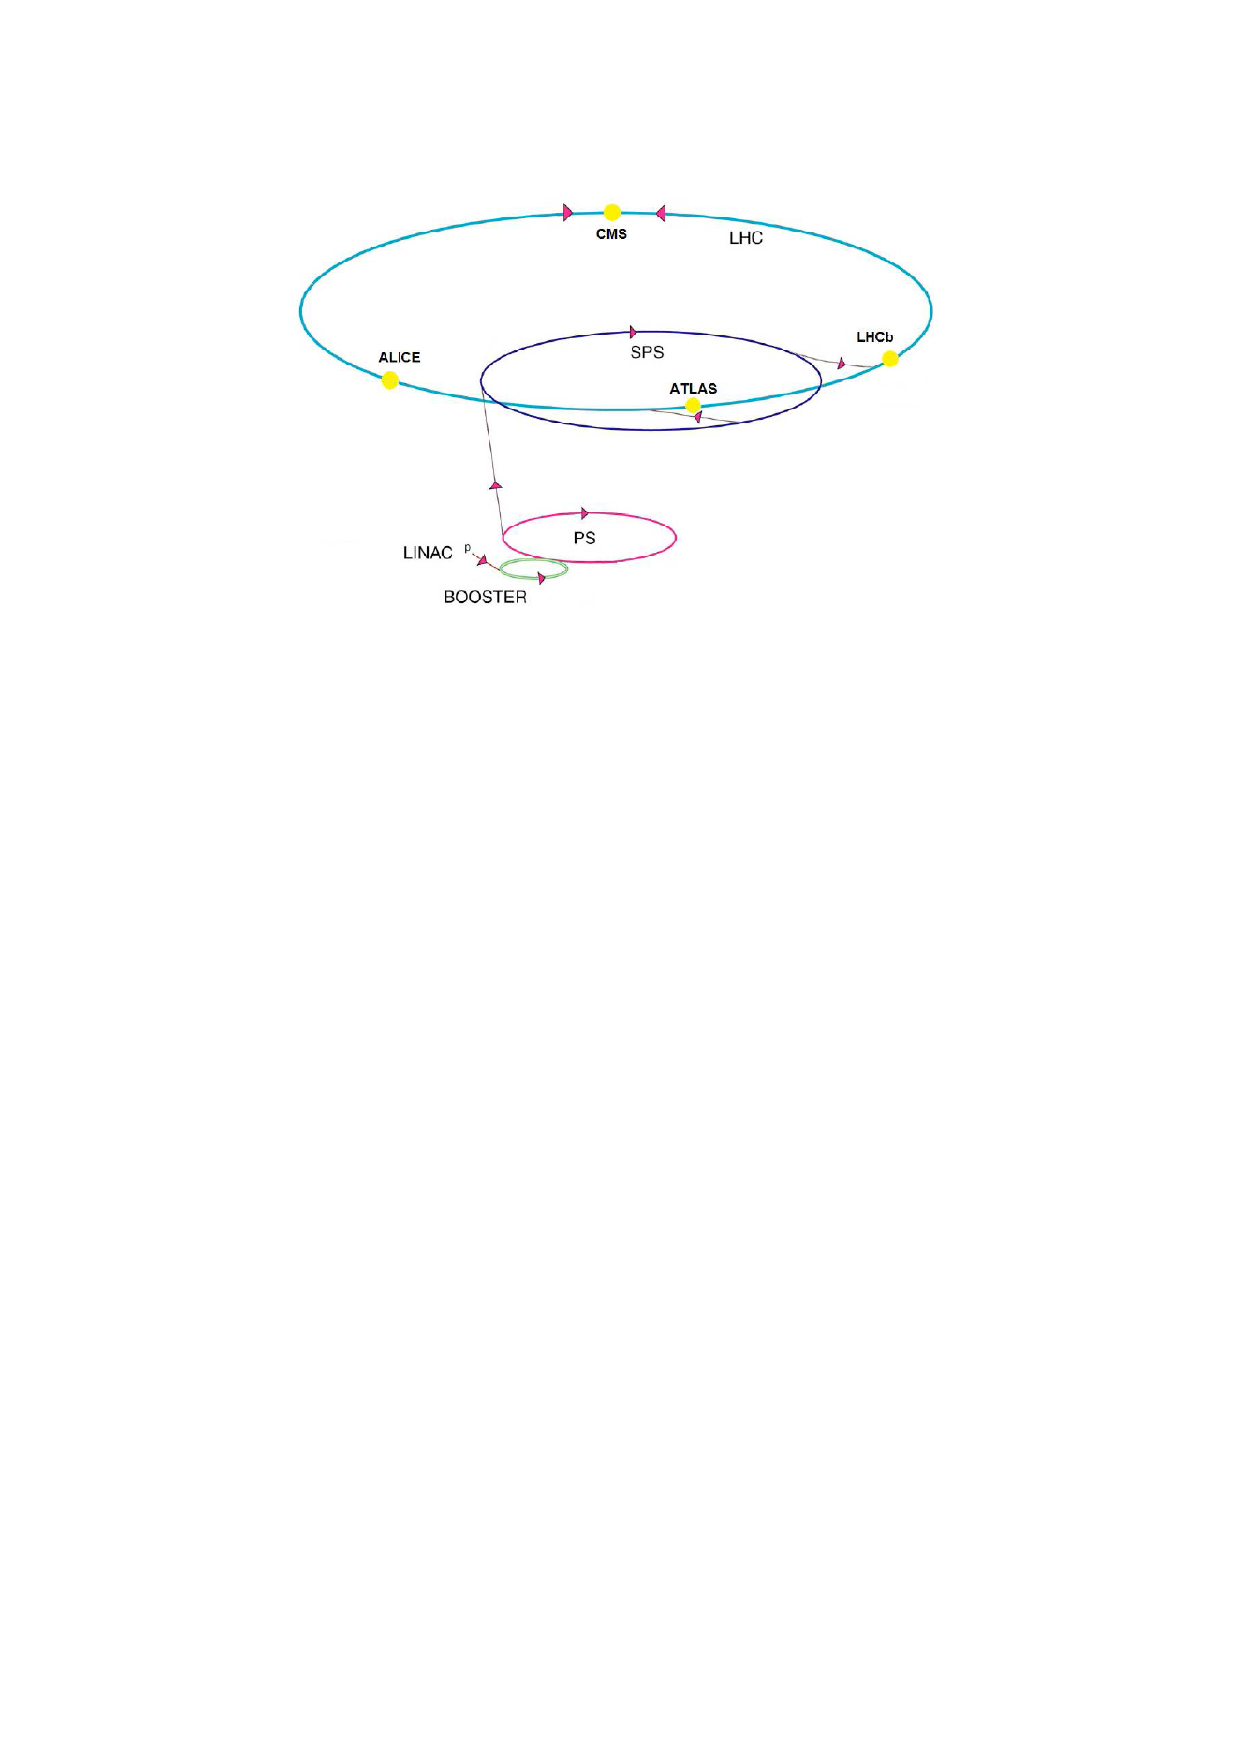
\includegraphics[width=\textwidth]{LHC.pdf}
\caption{A diagram of the LHC accelerator complex. Reproduced from
\cite{physics_tdr_1}.}
\label{fig:LHC}
\end{figure}

The CMS detector is one of the four general purpose LHC experiments. It was 
designed to explore O(TeV) energy proton-proton collisions for indications of 
physics beyond the Standard Model. The CMS detector is $21.6\unit{m}$ long and
$14.6\unit{m}$ in diameter and has a total weight of 13 500 tonnes. It is 
located at Point 5 on the LHC ring near Cessy in France. Figure \ref{fig:CMS} 
shows the layout of the CMS detector. \\

\begin{figure}
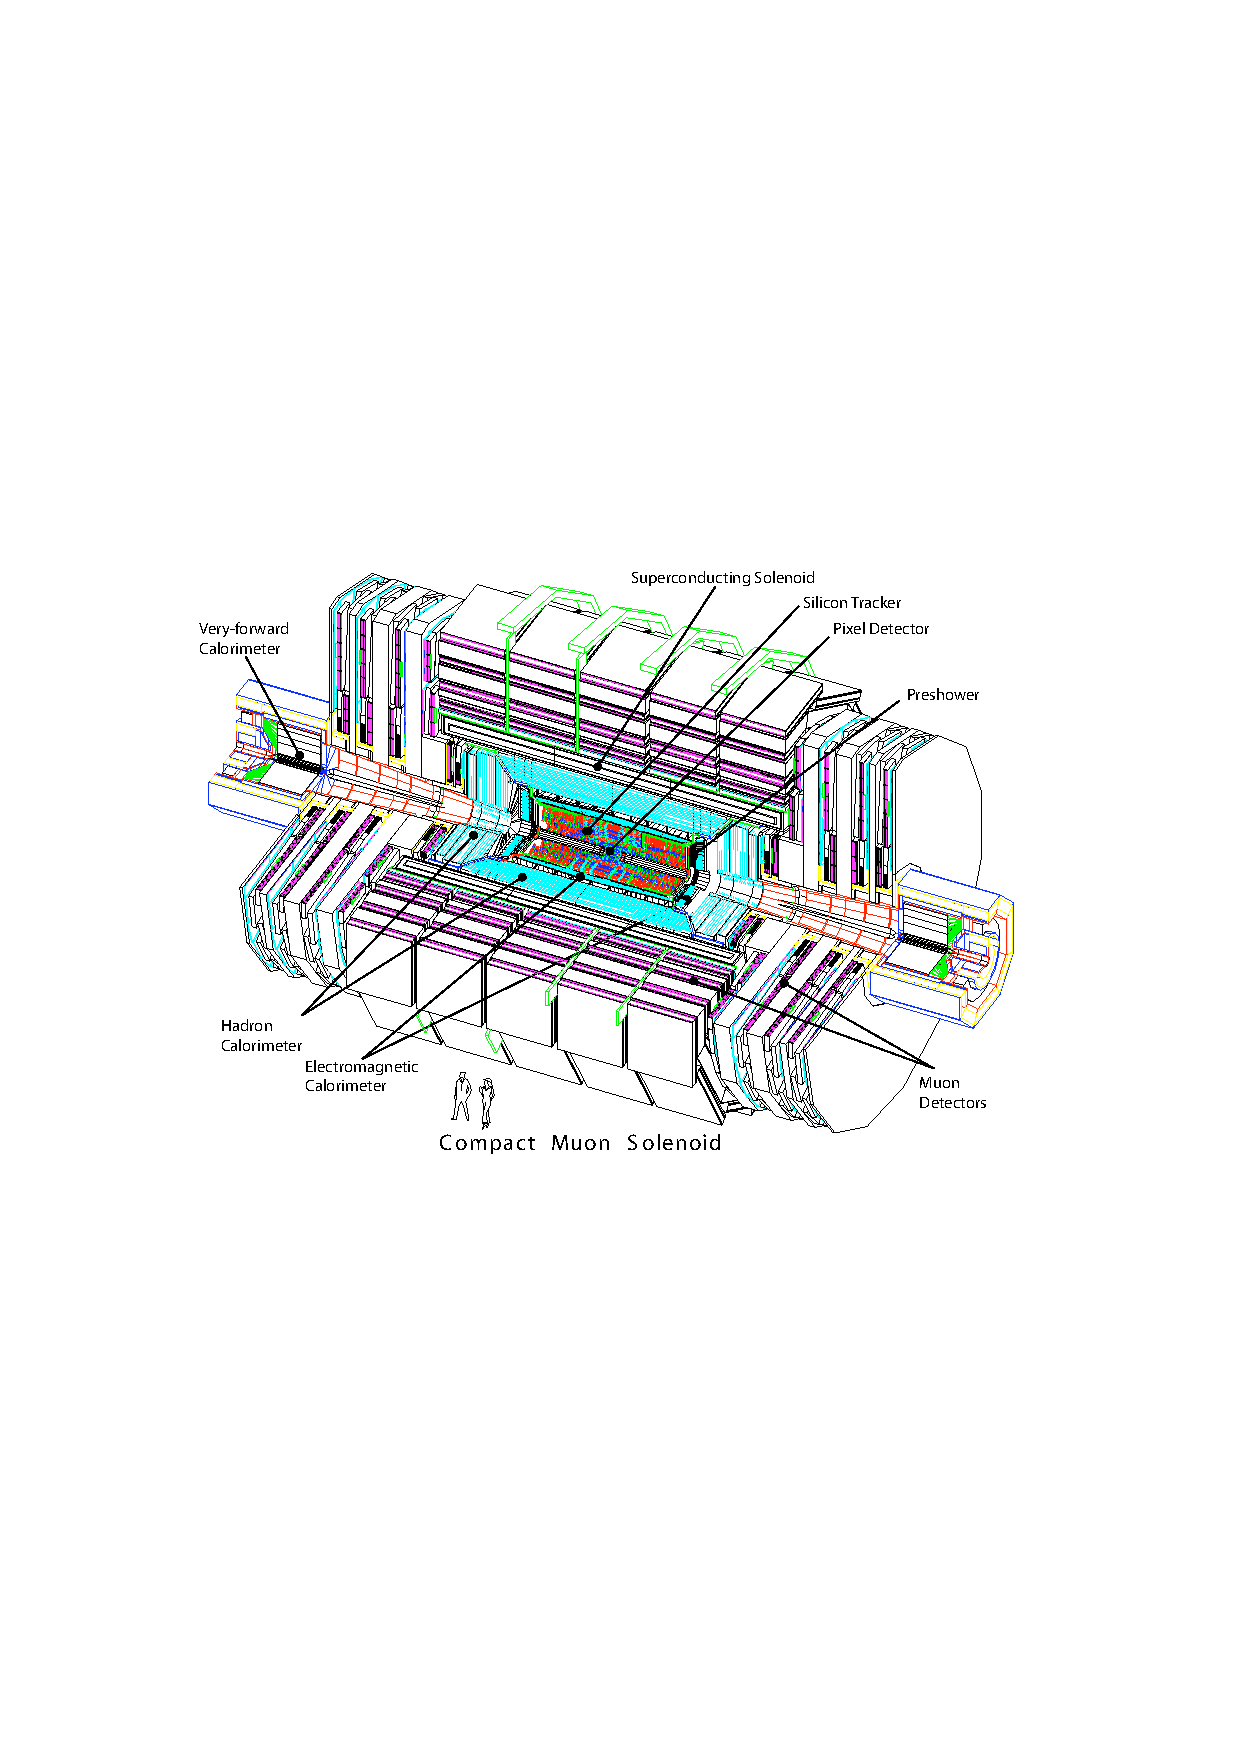
\includegraphics[width=\textwidth]{CMS.pdf}
\caption{A view of the layers inside the CMS detector. Reproduced from
\cite{physics_tdr_1}.}
\label{fig:CMS}
\end{figure}

In the following sections each component of the CMS detector is described 
starting from the innermost and going to the outermost. The CMS trigger and the
computing model are also described. 

\section{Pixel Detector}

The pixel detector consists of 3 barrel layers with 2 endcap disks on each side
(Figure \ref{fig:Pixel}). The barrel layers are at mean radii of $4.4\unit{cm}$,
$7.3\unit{cm}$ and $10.2\unit{cm}$ and have a length of $53\unit{cm}$. The 
endcap disks are placed either side at $|z| = 34.5\unit{cm}$ and 
$46.5\unit{cm}$. \\

\begin{figure}
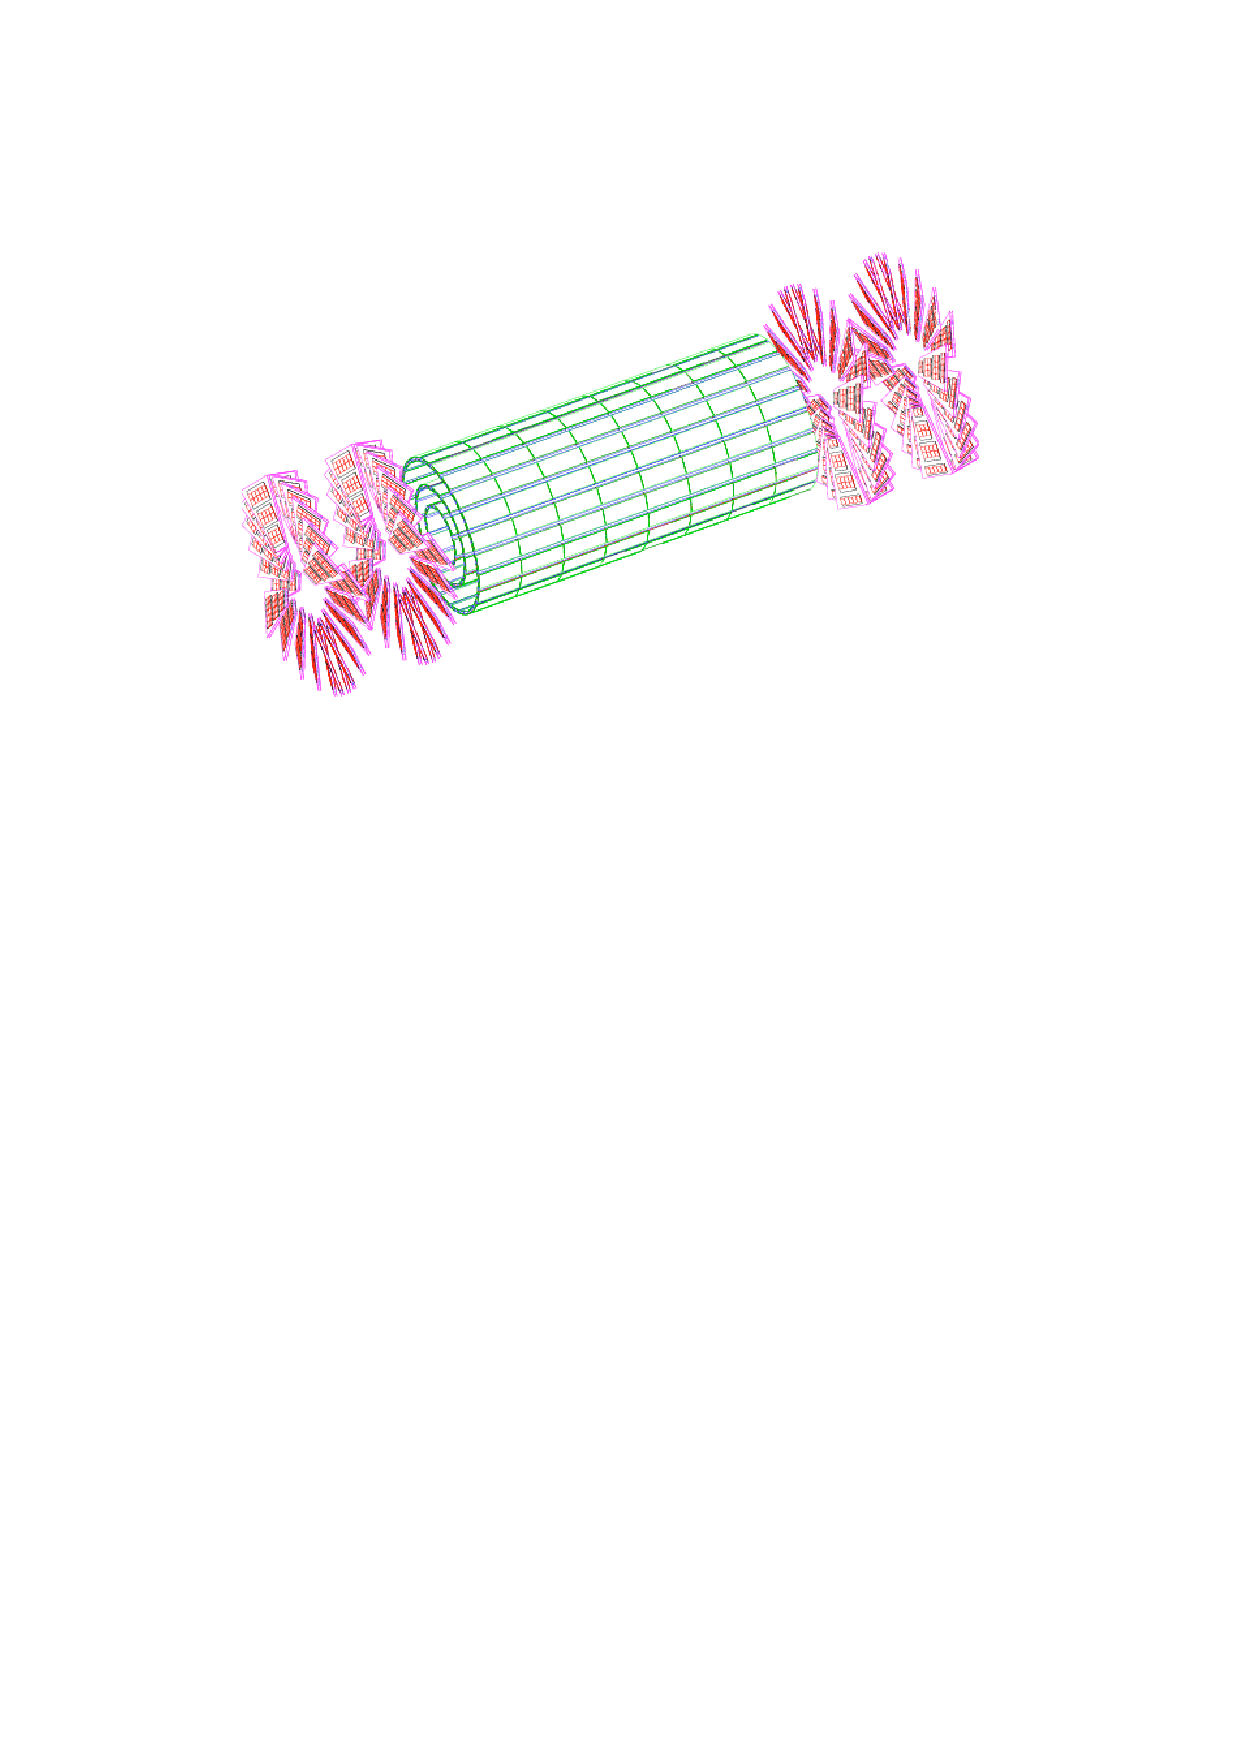
\includegraphics[width=\textwidth]{Pixel.pdf}
\caption{A diagram of the pixel detector. Reproduced from \cite{physics_tdr_1}.}
\label{fig:Pixel}
\end{figure}

The purpose of the pixel detector is to give good primary vertex resolution and
to initiate track reconstruction. The pixel size is $100\times150\unit{\mu m}$. 
The spatial resolution is about $10\unit{\mu m}$ for the (r,$\phi$) measurement 
and about $20\unit{\mu m}$ for the z measurement. \\

The primary vertex is found by clustering selected tracks in z. A fit is
performed based on a weight assigned to each track which is between 0 and 1
depending on the compatibility with the vertex \cite{primary_vertex}. \\

The primary vertex resolution depends strongly on the number of tracks in the
fit. Figure \ref{fig:primary_vertex} shows the primary vertex resolution as a
function of the number of tracks for various average track $\pT$ ranges.

\begin{figure}
\begin{center}
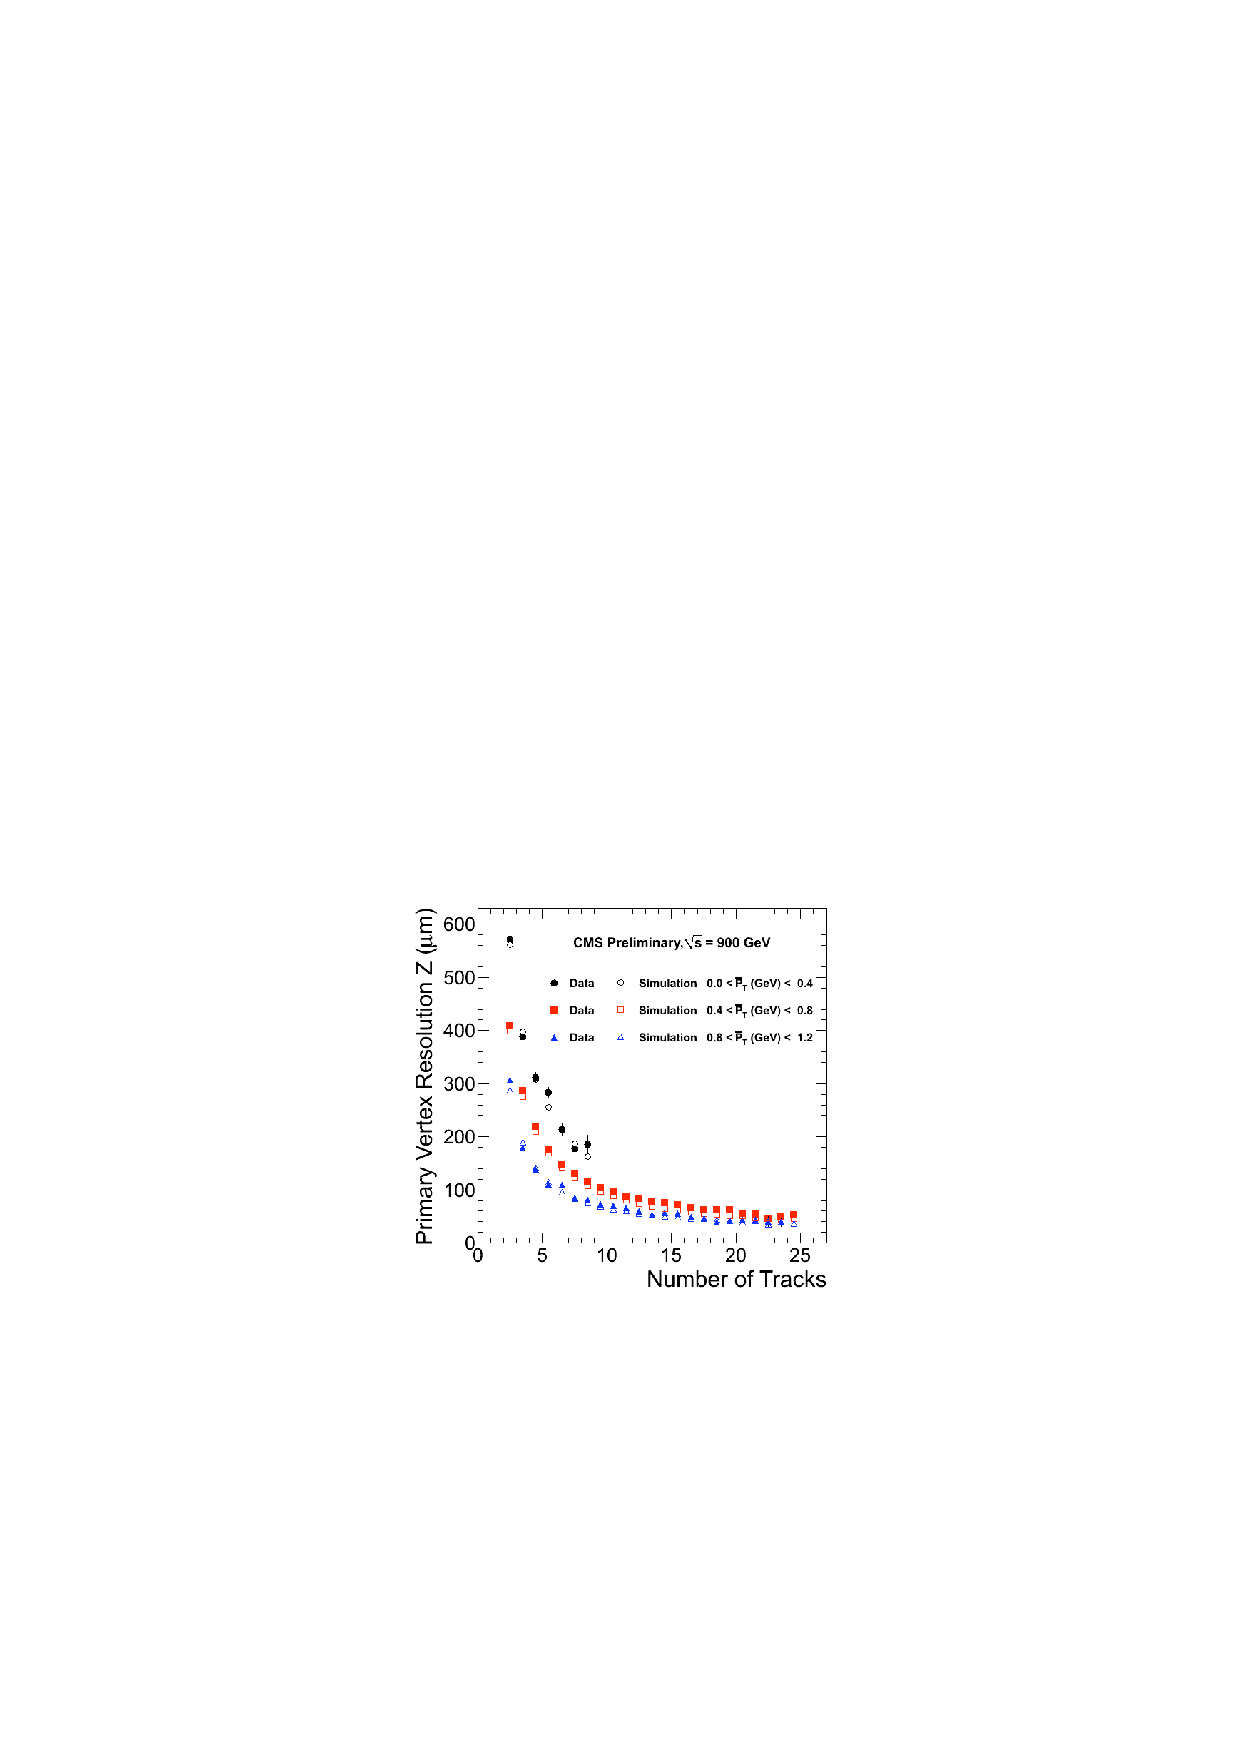
\includegraphics[width=\textwidth]{primary_vertex_resolution.pdf}
\end{center}
\caption{The Primary Vertex resolution as a function of the number of tracks for
various average track $\pT$ ranges. Reproduced from \cite{primary_vertex}.}
\label{fig:primary_vertex}
\end{figure}

\section{Silicon Strip Tracker}

The silicon strip tracker is designed to measure the trajectory of charged 
particles. It is made from strips of silicon which charged particles ionise. The
technology is the pn junction with a reverse bias voltage applied, which creates
a depletion region. Charged particles ionise inside the depleted region creating
electron hole pairs which travel to the electrodes where they form a signal. 
Silicon is used because it produces fast, radiation hard electronics and good
resolution. \\
  
The transverse momentum of a particle is measured from the curvature of the 
track in the magnetic field by Equation \ref{eq:pt_measurement}, where $\pT$ is
the transverse momentum in GeV, B is the magnetic field in Tesla and r is the
radius of curvature in metres. Only the hits are measured directly. The 
``sagitta'' or distance s in Figure \ref{fig:curvature} is deduced and the 
transverse momentum is calculated from this. Since s is inversely proportional 
to $\pT$, the resolution is worse at higher $\pT$.

\begin{equation}
\pT = 0.3Br
\label{eq:pt_measurement}
\end{equation}

\begin{figure}
\begin{center}
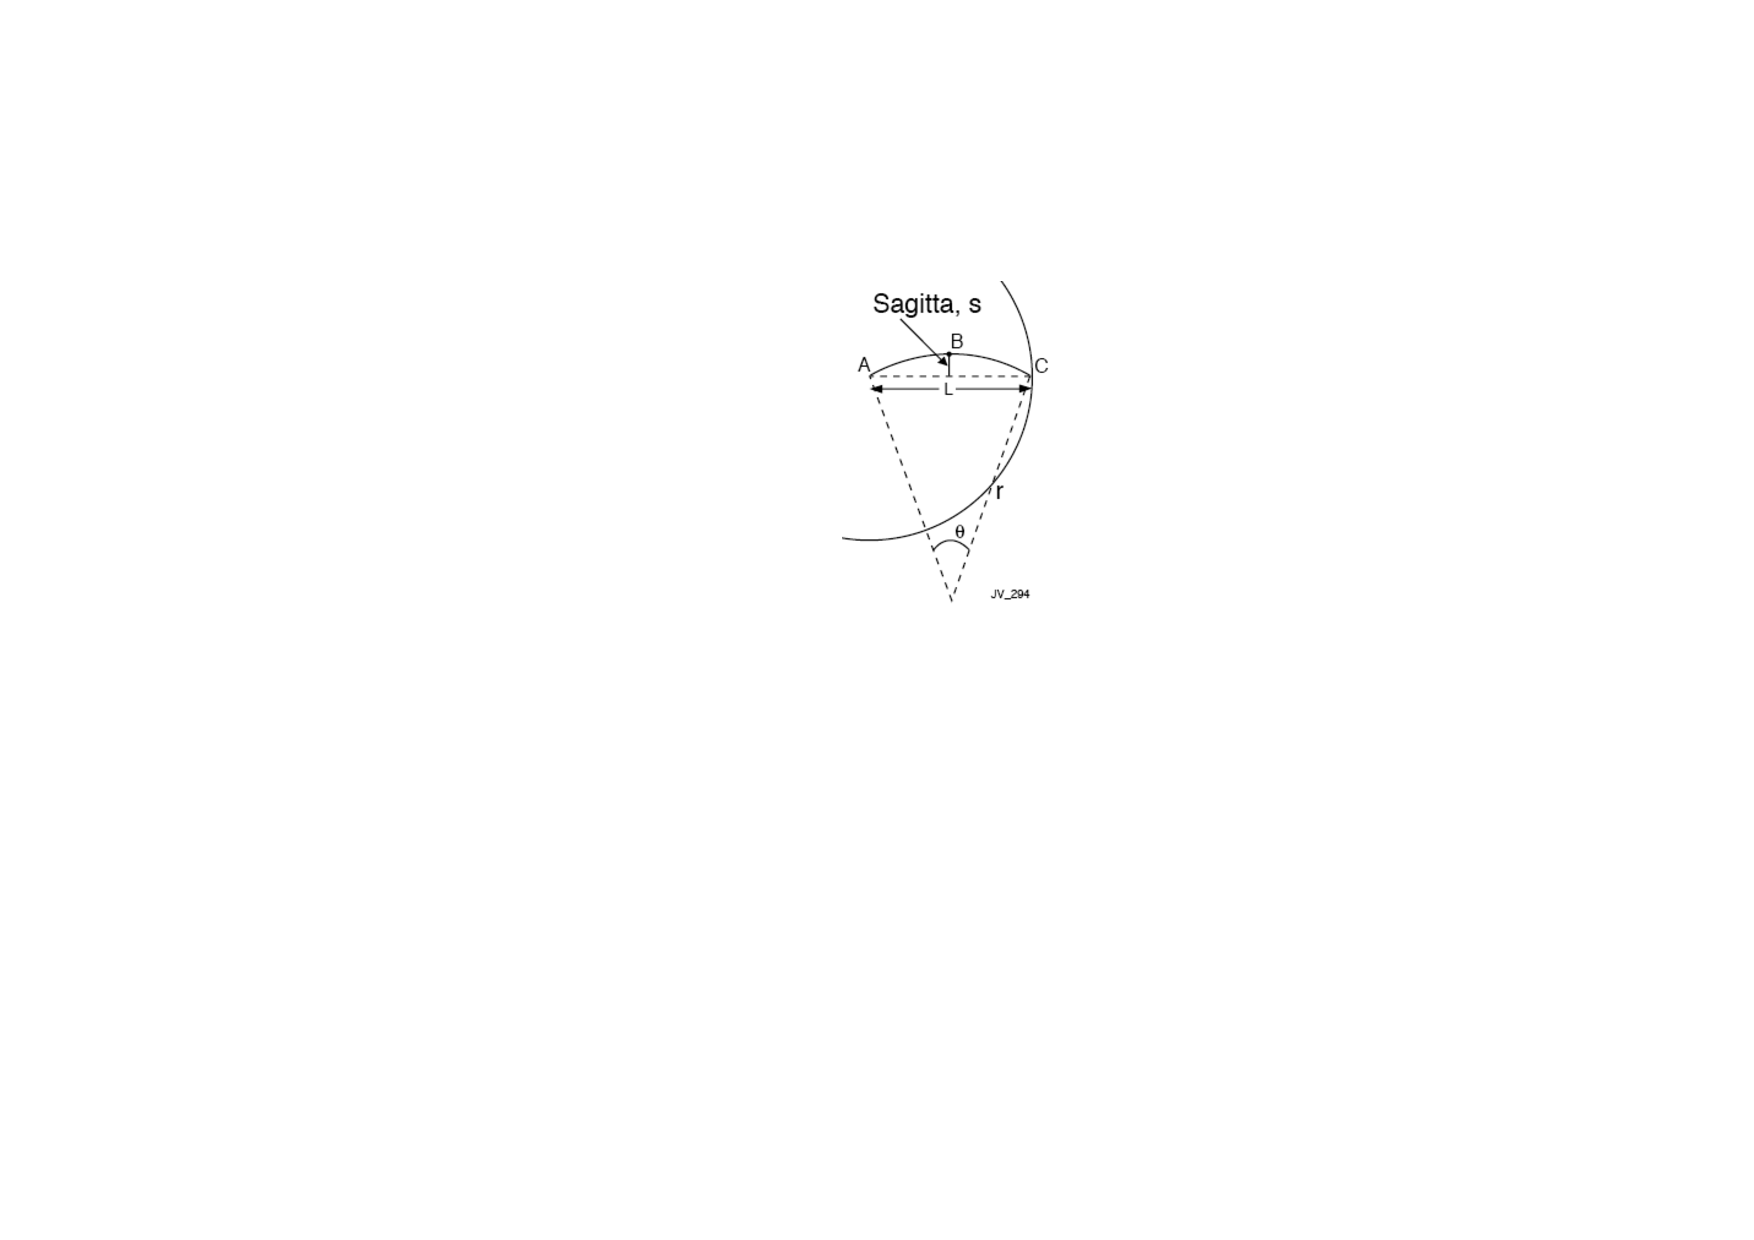
\includegraphics[width=0.3\textwidth]{Curvature.pdf}
\end{center}
\caption{Diagram illustrating how the transverse momentum is calculated from the
curvature of the track in the magnetic field.}
\label{fig:curvature}
\end{figure}

The silicon strip tracker is made up of 4 sub-detectors: the Tracker Inner 
Barrel (TIB), the Tracker Outer Barrel (TOB), the Tracker Endcap (TEC) and the
Tracker Inner Disks (TID). Figure \ref{fig:Silicon_Strip_Tracker} shows the 
layout of the tracker. \\

\begin{figure}
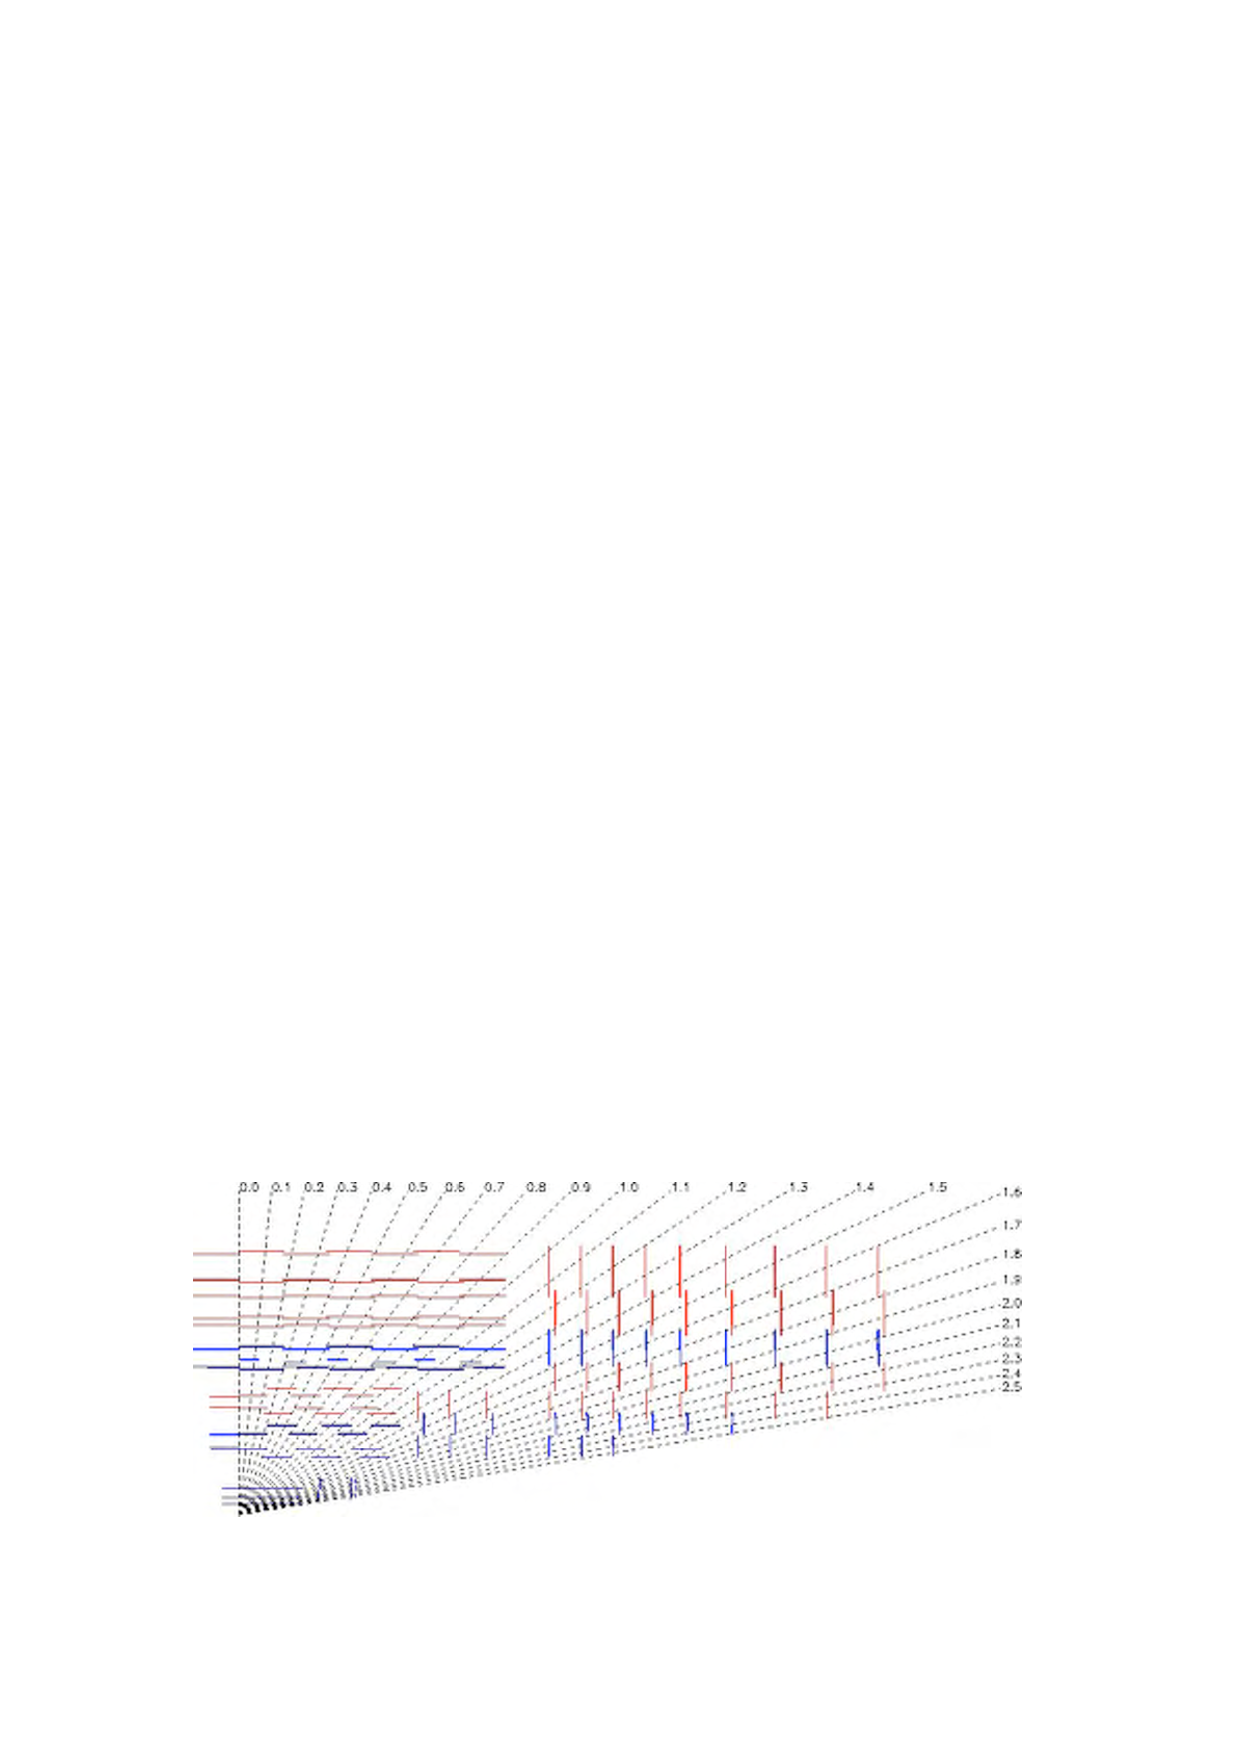
\includegraphics[width=\textwidth]{Silicon_Strip_Tracker.pdf}
\caption{The layout of the silicon strip tracker. Reproduced from 
\cite{physics_tdr_1}.}
\label{fig:Silicon_Strip_Tracker}
\end{figure}

The resolution of the tracker is shown for muons of $p_{T} = 1$, 10 and $100 
\unit{GeV}$ in Figure \ref{fig:tracker_resolution}.

\begin{figure}
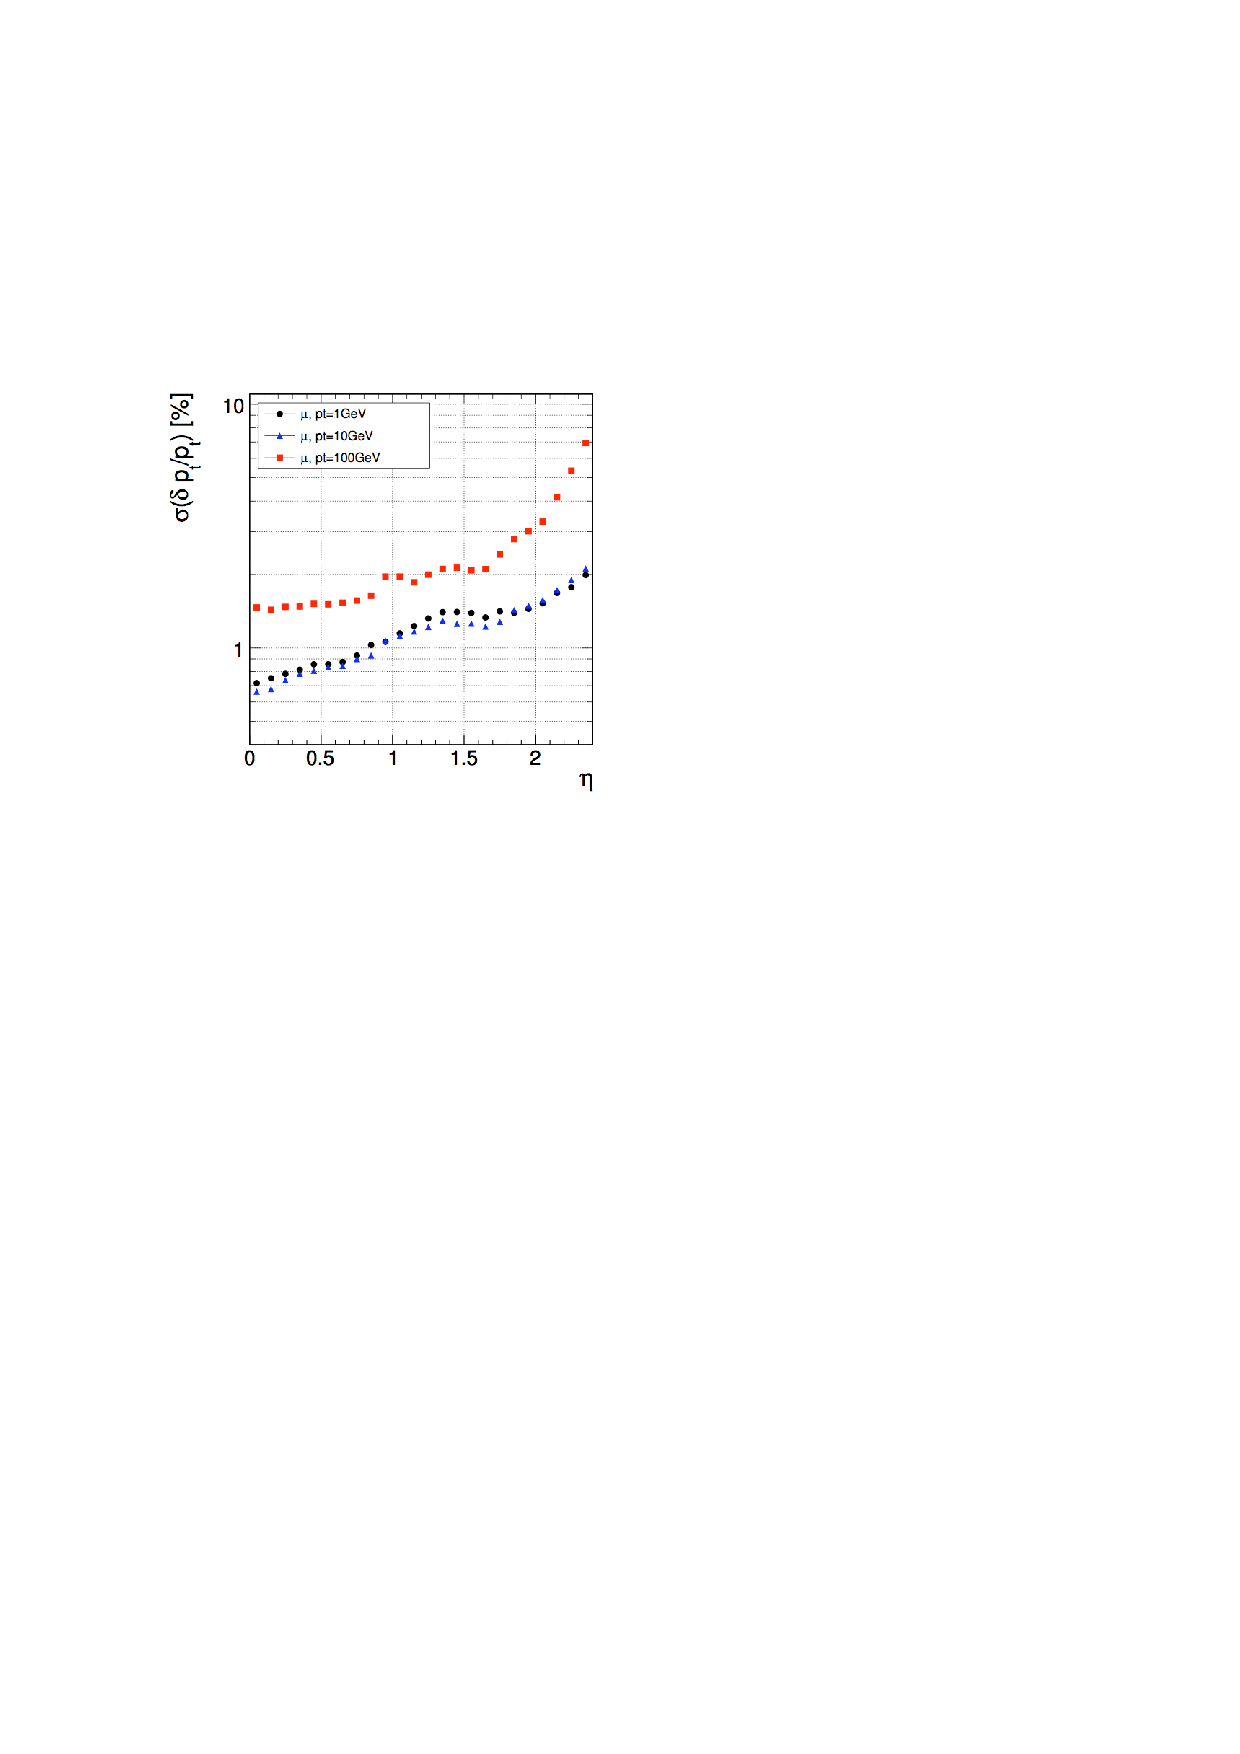
\includegraphics[width=\textwidth]{Tracker_Resolution.pdf}
\caption{The resolution of the tracker as a function of $\eta$ for muons of
$p_{T} = 1$, 10 and $100 \unit{GeV}$.}
\label{fig:tracker_resolution}
\end{figure}

\section{Electromagnetic Calorimeter}

The Electromagnetic Calorimeter (ECAL) is designed to measure the energy of
electromagnetic showers from photons, electrons and $\pi^{0}$s. It must provide
good energy resolution and good containment of the electromagnetic shower. \\

\begin{figure}
\begin{center}
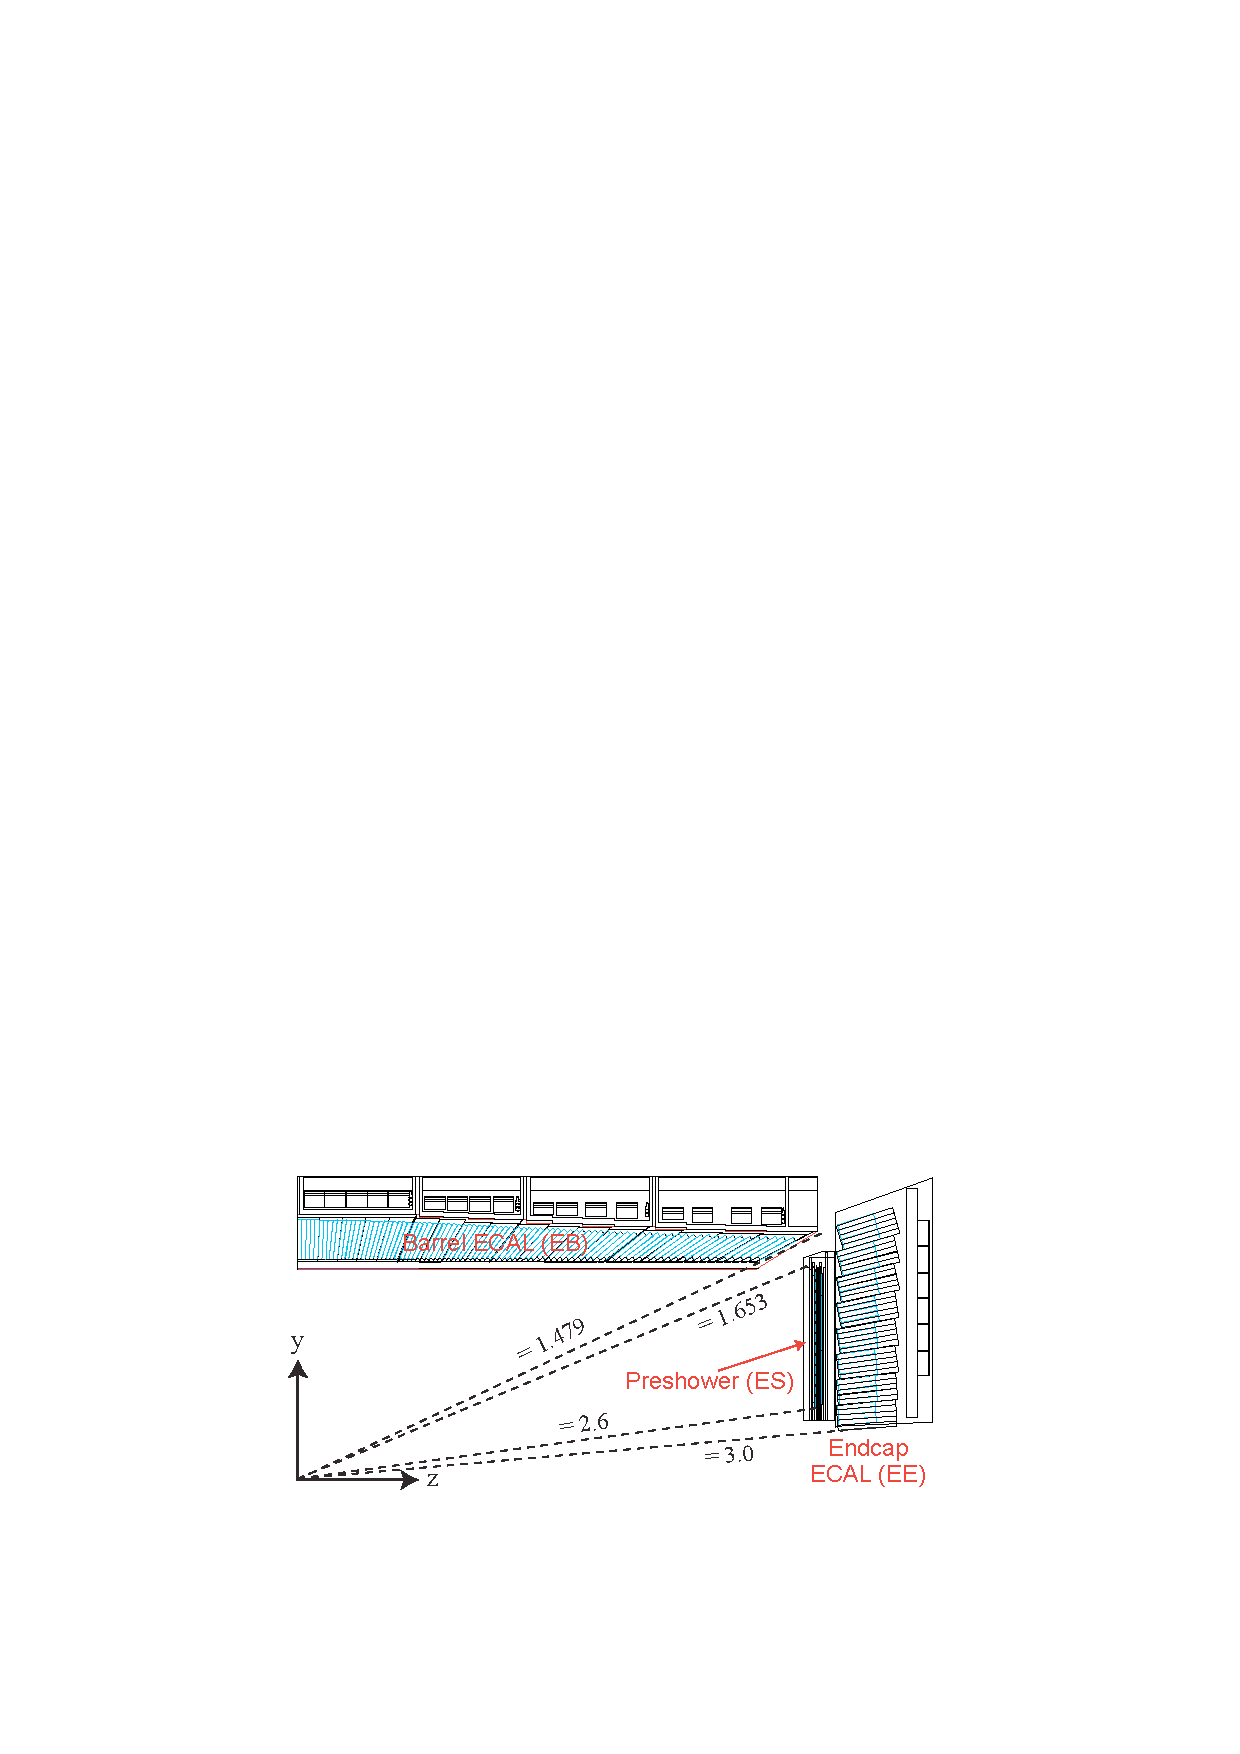
\includegraphics[width=\textwidth]{ECAL.pdf}
\end{center}
\caption{A diagram of the layout of the ECAL.}
\label{fig:ECAL}
\end{figure}

The ECAL has 3 components: the ECAL barrel (EB), the ECAL endcap (EE) and the
ECAL pre-shower (ES). The EB covers the range $|\eta| < 1.479$. The EB radius is
1.29m and the total length in the z-direction is 6m. The EE consists of two 
identical detectors on either side of the EB covering the region $1.479 < |\eta|
< 3$. The ES is positioned in front of the EE to improve the $\gamma$/$\pi^{0}$ 
discrimination which is important for $H\rightarrow\gamma\gamma$ searches. 
Figure \ref{fig:ECAL} shows a diagram of the layout of the ECAL. \\

\begin{figure}
\begin{center}
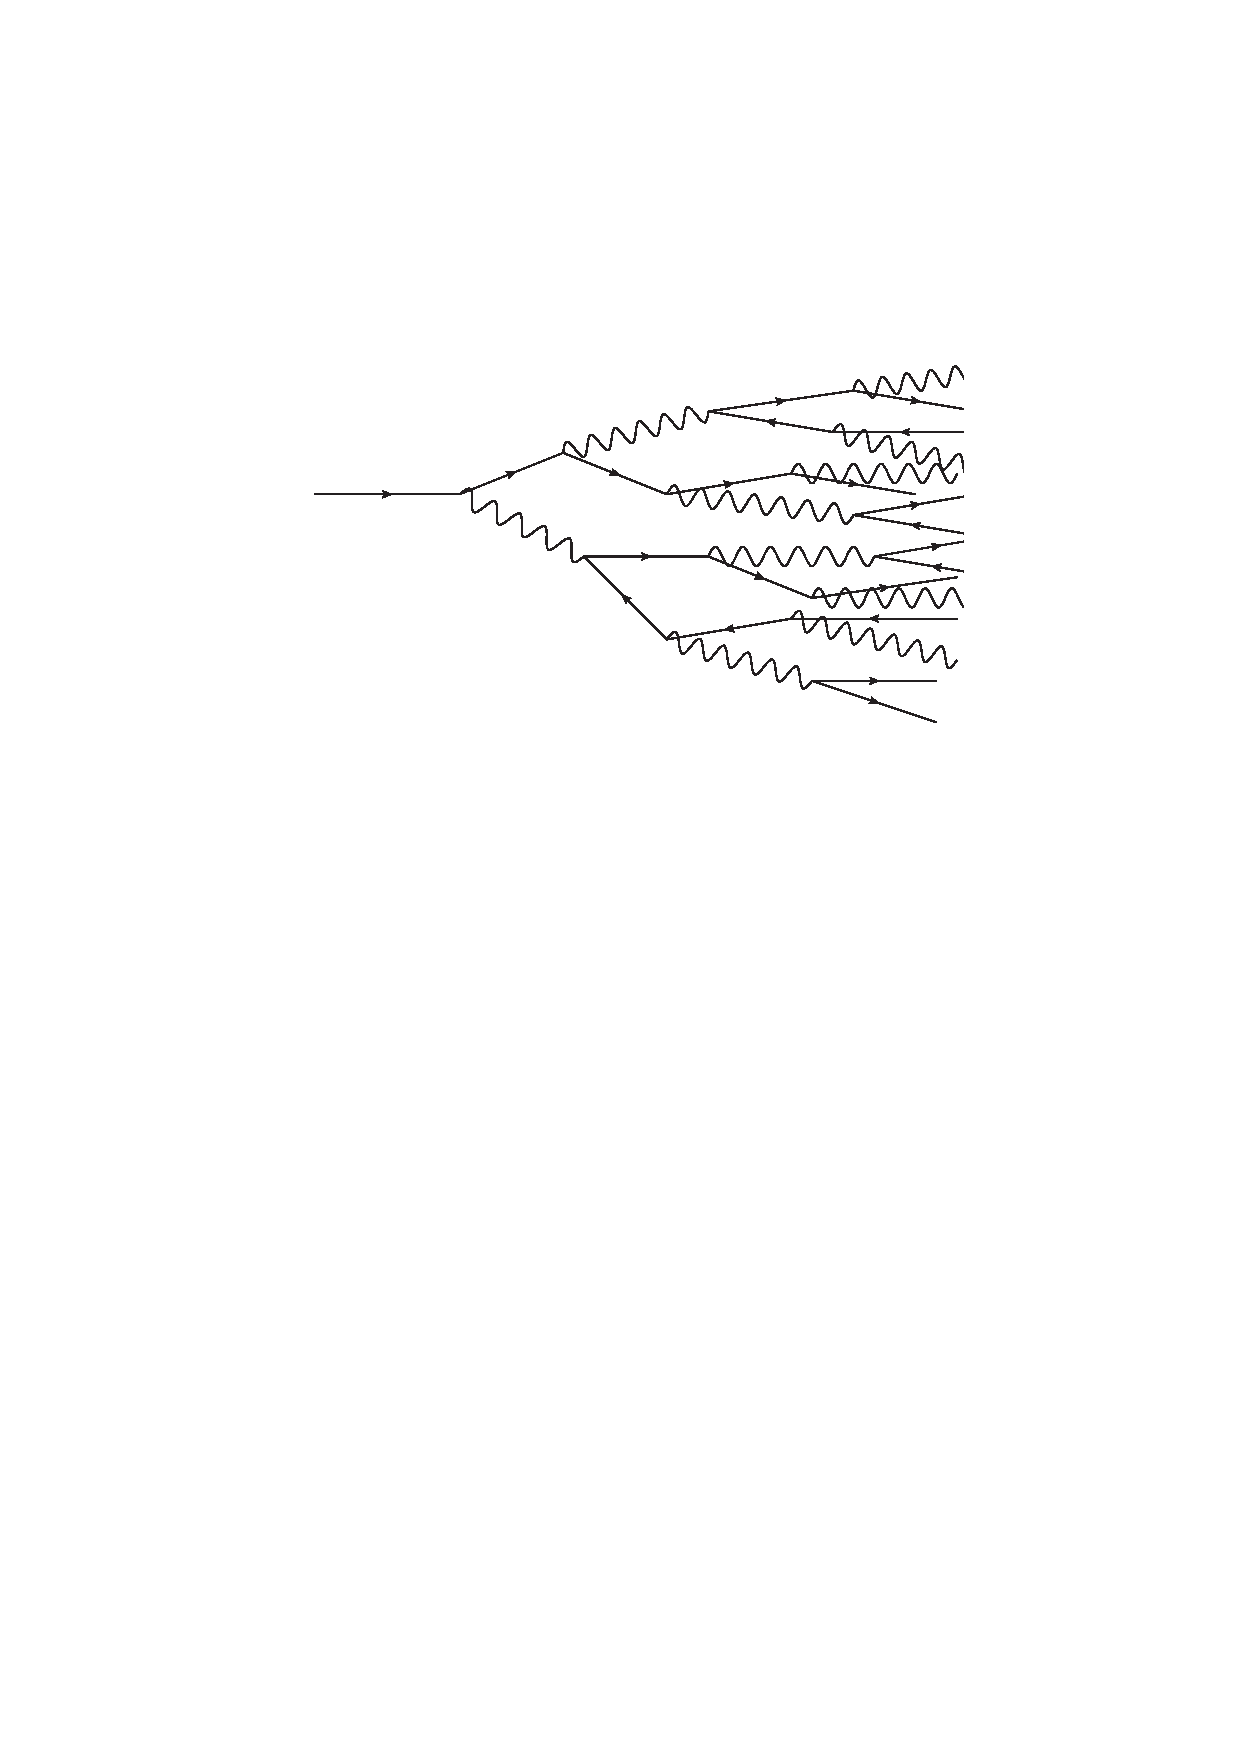
\includegraphics[width=0.7\textwidth]{EM_Shower.pdf}
\end{center}
\caption{An illustration of the development of an EM shower.}
\label{fig:em_shower}
\end{figure}

An electromagnetic shower progresses through two processes {\bf bremsstrahlung},
where an electron or positron emits a photon, and {\bf pair production}, where a
photon converts to an electron and a positron. Figure \ref{fig:em_shower} shows
how an electromagnetic shower progresses. The shower continues until the
electrons/photons reach a critical energy, $E_{c}$, where no more particles are 
produced as the dominant energy losses are through Compton scattering and
photoelectric effect for photons and ionisation for electrons. \\

The calorimeter measures the energy. have a heavy material that initiates the shower and a scintillation
material which converts it to a light signal. Sampling calorimeters are in
layers with layers of heavy material to initiate the shower and layers of
scintillator to sample the shower. In homogeneous calorimeters the heavy
material and the scintillator are one and the same. Materials have two
characteristic lengths which describe the shape of EM showers. Radiation length
is the length over which an electron or photon's energy is reduced to 1/e of
it's initial energy. Moliere radius describes the lateral size of the shower; it
is the radius which contains 90\% of the energy of the shower. \\  

The EB and EE are homogeneous calorimeters made of lead tungstate ($PbWO_{4}$)
crystals. This material was chosen because of its short radiation length ($X_{0}
= 0.89\unit{cm}$) and short Moliere radius ($r_{m} = 2.2\unit{cm}$). The 
crystals have a low light yield. The scintillation light is blue/green with a 
maximum at $420-430\unit{nm}$. The light is detected by Avalanche Photodiodes 
(APDs) in the EB and Vacuum Phototriodes (VPTs) in the EE. The choice of 
photodetectors was based on the requirement of adequate electronic gain given 
the low light yield of the crystals, operation in the magnetic field and 
radiation tolerence for the enivonment in which they operate. \\

In the EB the length of the crystals is $23\unit{cm}$ (26 $X_{0}$) and the 
cross-section is $0.0147\times0.0147$ in $\eta$-$\phi$ or about 
$22\unit{mm}\times22\unit{mm}$ at the front face. Figure \ref{fig:ECAL} shows 
the layout of crystals in the EB. The crystals are angled at $3^{o}$ with 
respect to the interaction point. To minimise the risk of particles escaping 
down the cracks between the crystals. The ECAL is divided into regions called 
Trigger Towers (TTs) for which trigger primitives (crystal energy sums) used by 
the trigger are calculated. There are $85\times72$ TTs in the EB each consisting 
of 5x5 arrays of crystals. \\

In the EE the length of the crystals is $22\unit{cm}$ ($25X_{0}$). Due to the 
geometry of the detector the granularity in $\eta$-$\phi$ varies across the EE. 
\\

The ES is a sampling calorimeter made of lead to initiate the shower and
silicon strip sensors to sample the shower. It has a depth of $20\unit{cm}$ 
($3X_{0}$). \\

The energy resolution, $\sigma$, has been parameterised as a function of energy 
in Equation \ref{eq:ECAL_Resolution}. 

\begin{equation}
\left( \frac{\sigma}{E} \right)^{2} = \left( \frac{S}{\sqrt{E}} \right)^{2} +
\left( \frac{N}{E} \right)^{2} + C
\label{eq:ECAL_Resolution}
\end{equation}

The parameters S, N and C represent the stochastic term, the noise term and the
constant term respectively. \\

The stochastic term, $S$, is related to the uncertainty in the number of photons 
detected. The number of photons for a given energy electromagnetic shower 
follows a Poisson distribution. So if N photons are detected, the uncertainty is 
$\sqrt{N}$. And the energy is proportional to the number of photons, hence the 
$\sqrt{E}$ dependence of this term. \\

The noise term, $N$, is not energy dependent. The noise is about $20\unit{MeV}$ 
per crystal, or $100\unit{MeV}$ per trigger tower. \\

The constant term, $C$, contains those uncertainties which are proportional to
energy such as inter-calibration uncertainties. \\

Figure \ref{fig:ECAL_Energy_Resolution} shows the energy resolution of the ECAL
as a function of beam energy measured using the test beam \cite{test_beam}.

\begin{figure}
\begin{center}
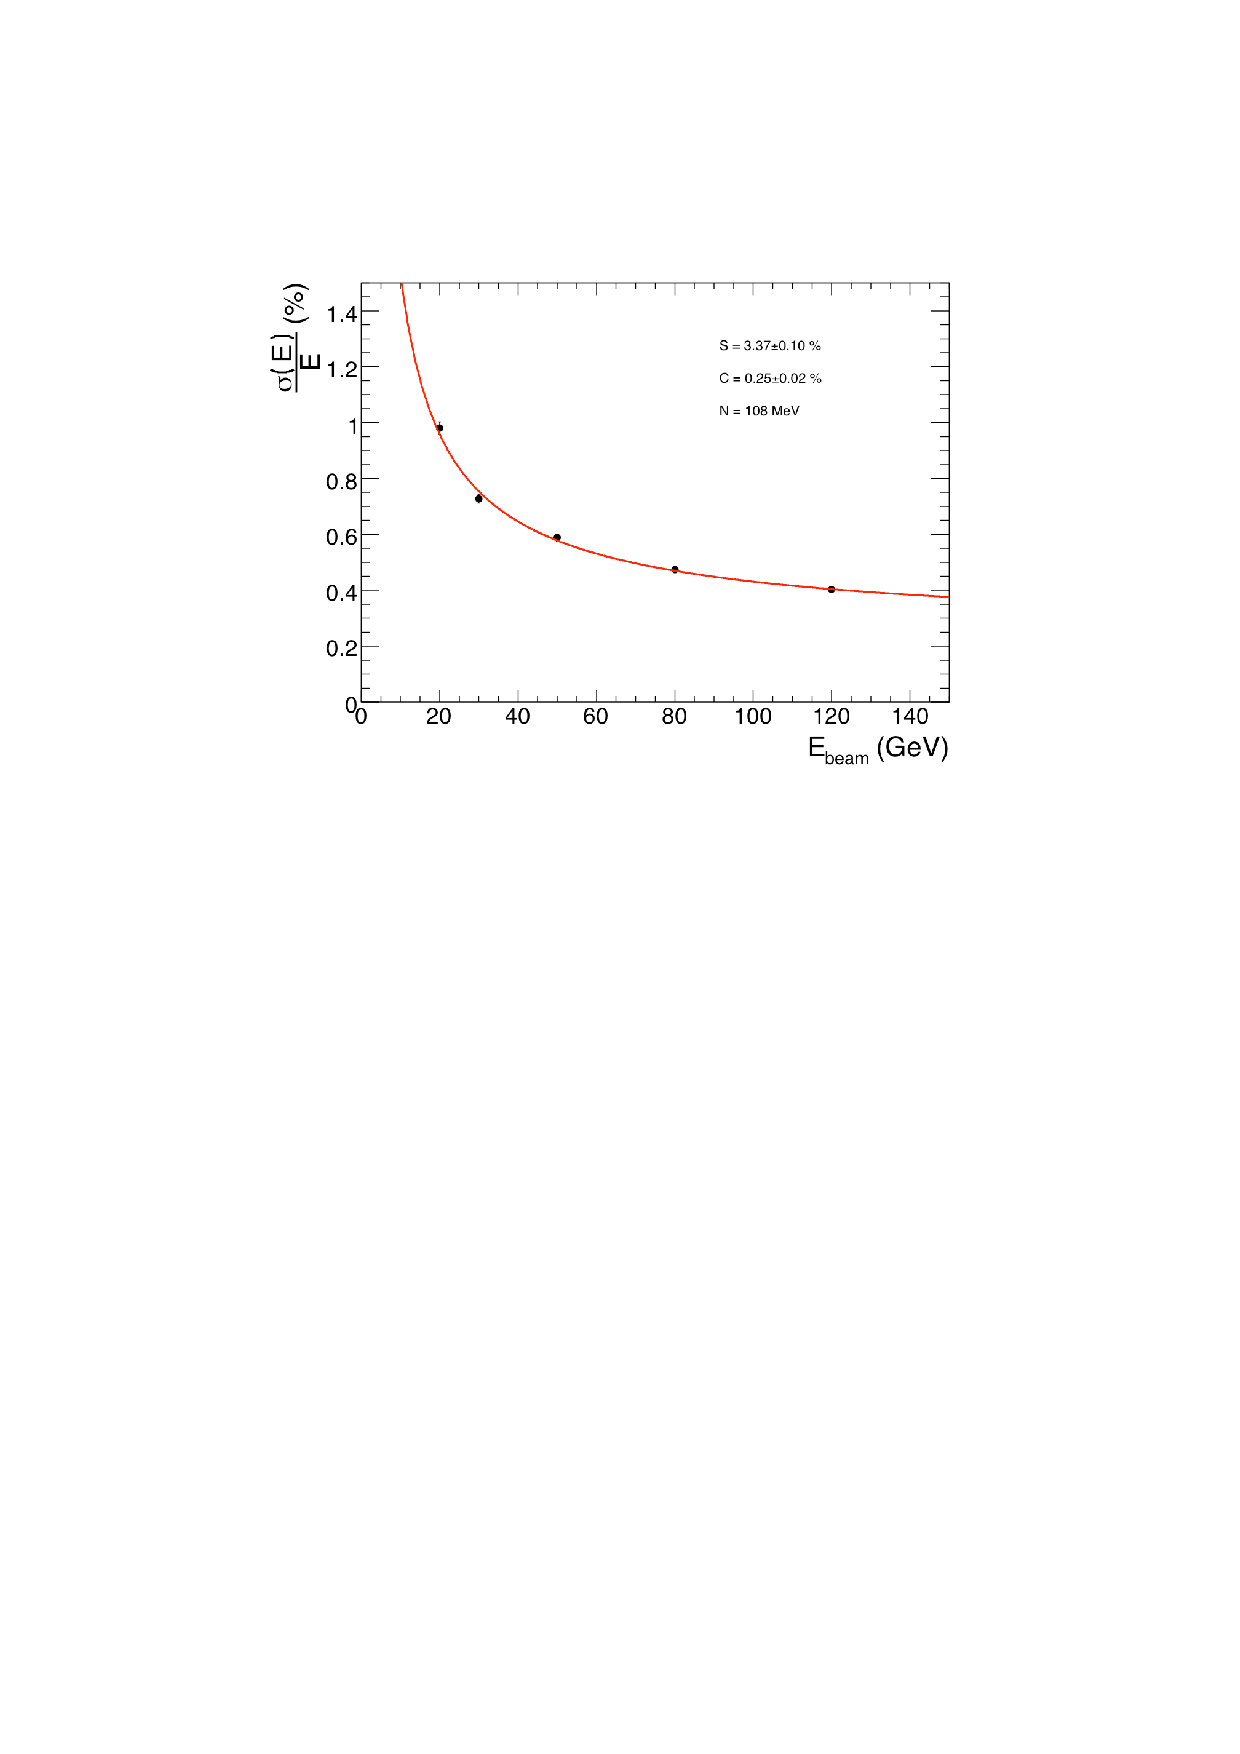
\includegraphics[width=0.7\textwidth]{ECAL_Energy_Resolution.pdf}
\end{center}
\caption{The energy resolution of the ECAL as a function of the beam energy as
measured using the test beam. The parameterisation of the resolution has been 
fitted and values extracted for the parameters. Reproduced from
\cite{test_beam}.}
\label{fig:ECAL_Energy_Resolution}
\end{figure}

\section{Hadronic Calorimeter}

The Hadronic Calorimeter (HCAL) measures the energy of hadronic showers and
assits in the triggering and measurement of jets and missing transverse energy.
\\

The HCAL covers the range $|\eta| < 5$ and consists of four subdetectors: the
Hadron Barrel (HB), the Hadron Outer (HO), the Hadron Endcap (HE) and the Hadron
Forward (HF). The HB covers the region $|\eta| < 1.4$ and contains towers with a 
granularity of $\Delta\eta\times\Delta\phi = 0.087\times0.087$. The HB is 
constrained radially to be between the ECAL outer surface (at r = 1.77m) and the
inner surface of the solenoid (at r = 2.95m). This constarins the amount of 
material that can be put in to absorb the hadronic showers. For this reason the 
HO lies outside the HB and the magnet in the region $|\eta| < 1.26$ and contains
extra scintillators to catch energy leakage from high energy jets. The HE covers
the range $1.3 < |\eta| < 3.0$ with a granularity that varies with $\eta$ from 
$\Delta\eta\times\Delta\phi = 0.087\times0.087$ at $\eta = 1.3$ to 
$\Delta\eta\times\Delta\phi = 0.350\times0.174$ at $\eta = 3.0$. The region $3 <
 |\eta| < 5$ is covered by the HF. \\

The HCAL is a sampling calorimeter with brass absorbers and plastic scintilator
tiles in the central and endcap regions and steel absorbers with quartz fibre 
scintillators in the forward region. Brass has a short interaction length () 
providing adequate containment within the limited space inside the magnet. Steel 
is used in the forward region due to its greater radiation tolerence. The 
scintillation light is detected by multi-channel hybrid photodiodes (HPDs) in 
the central region and photomultiplier tubes (PMTs) in the forward region. \\

\begin{figure}
\begin{center}
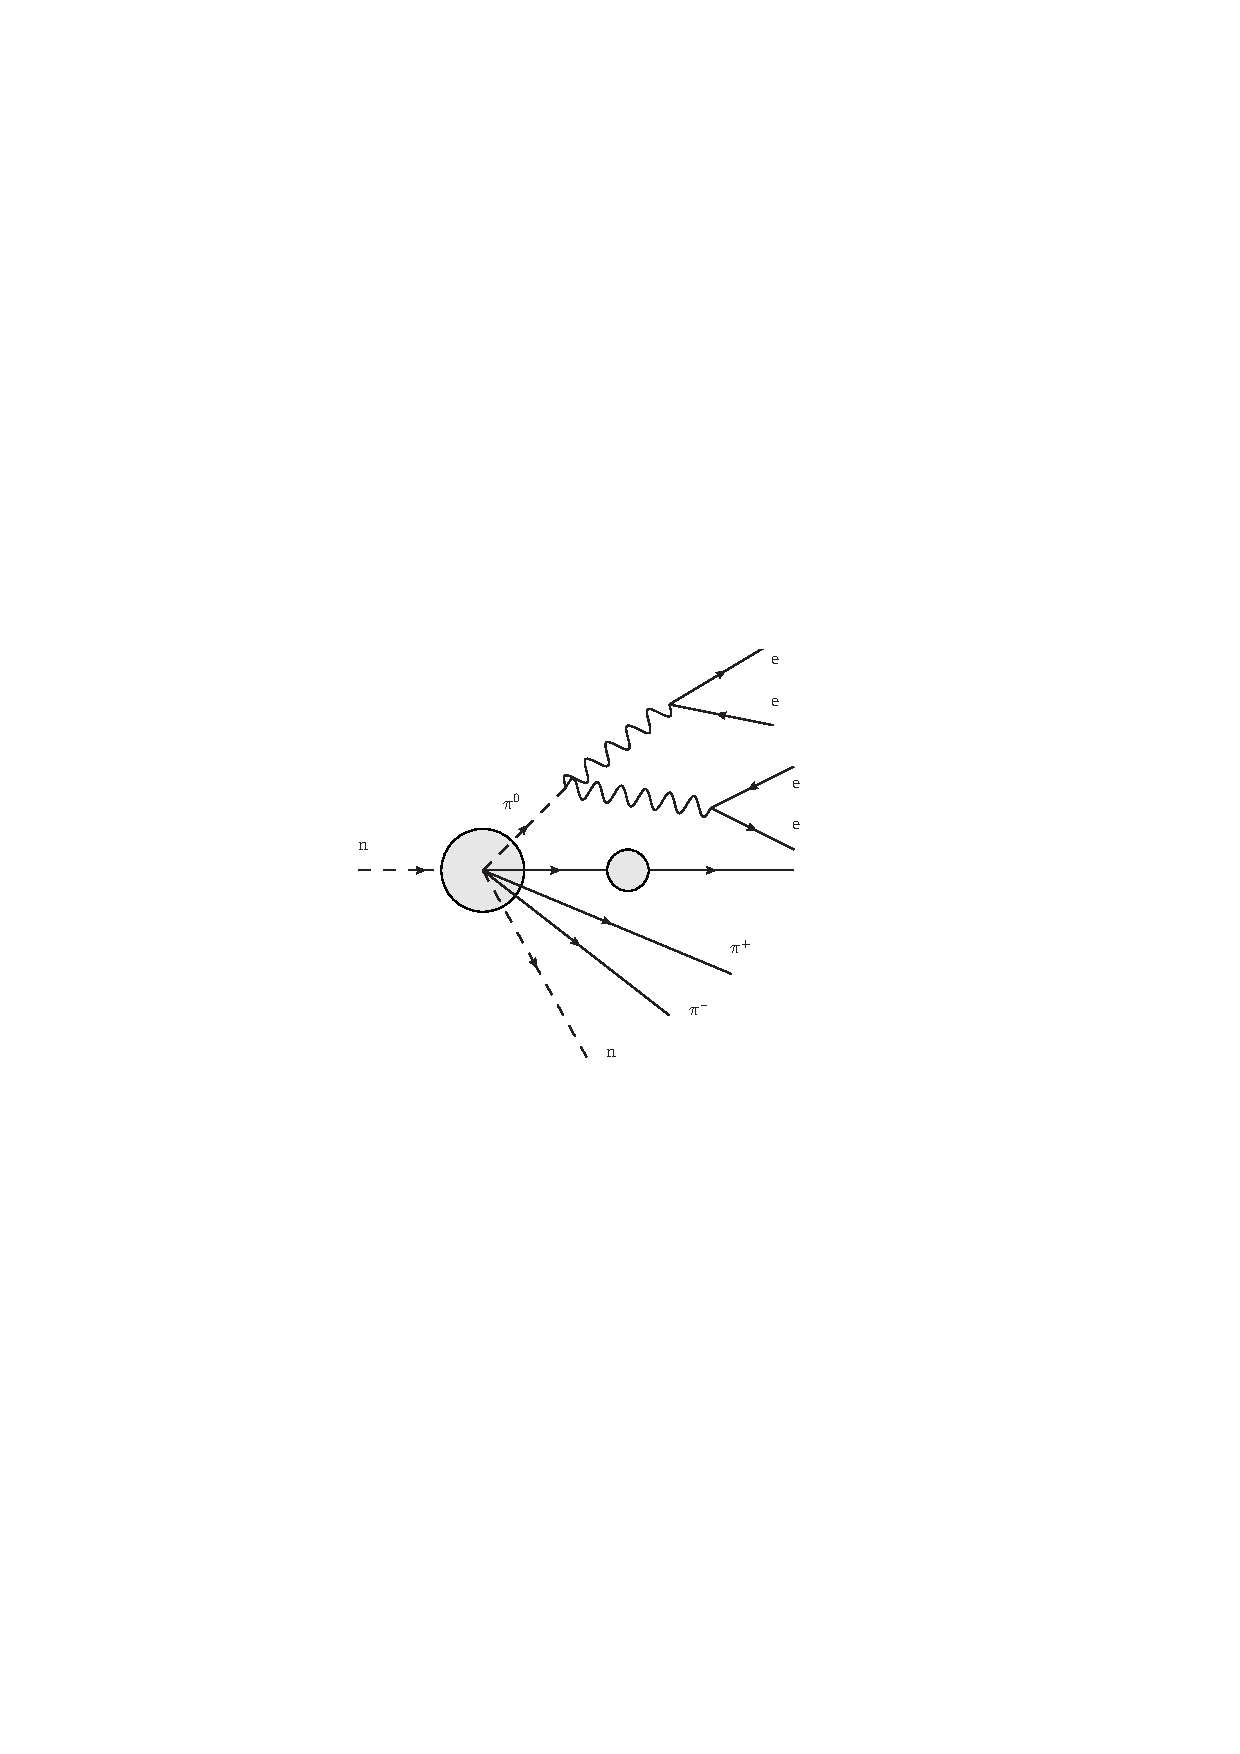
\includegraphics[width=0.7\textwidth]{Hadronic_Shower.pdf}
\end{center}
\caption{An illustration of the development of a hadronic shower.}
\label{fig:hadronic_shower}
\end{figure}

Figure \ref{fig:hadronic_shower} shows a diagram of the development of a
hadronic shower. \\

The jet energy resolution and the missing transverse energy resolution are the 
key indicators of the performance of the HCAL. Figure \ref{fig:jetmet} shows the
jet transverse energy resolution and the missing transverse energy resolution
\cite{jet_resolution, met_resolution}.

\begin{figure}
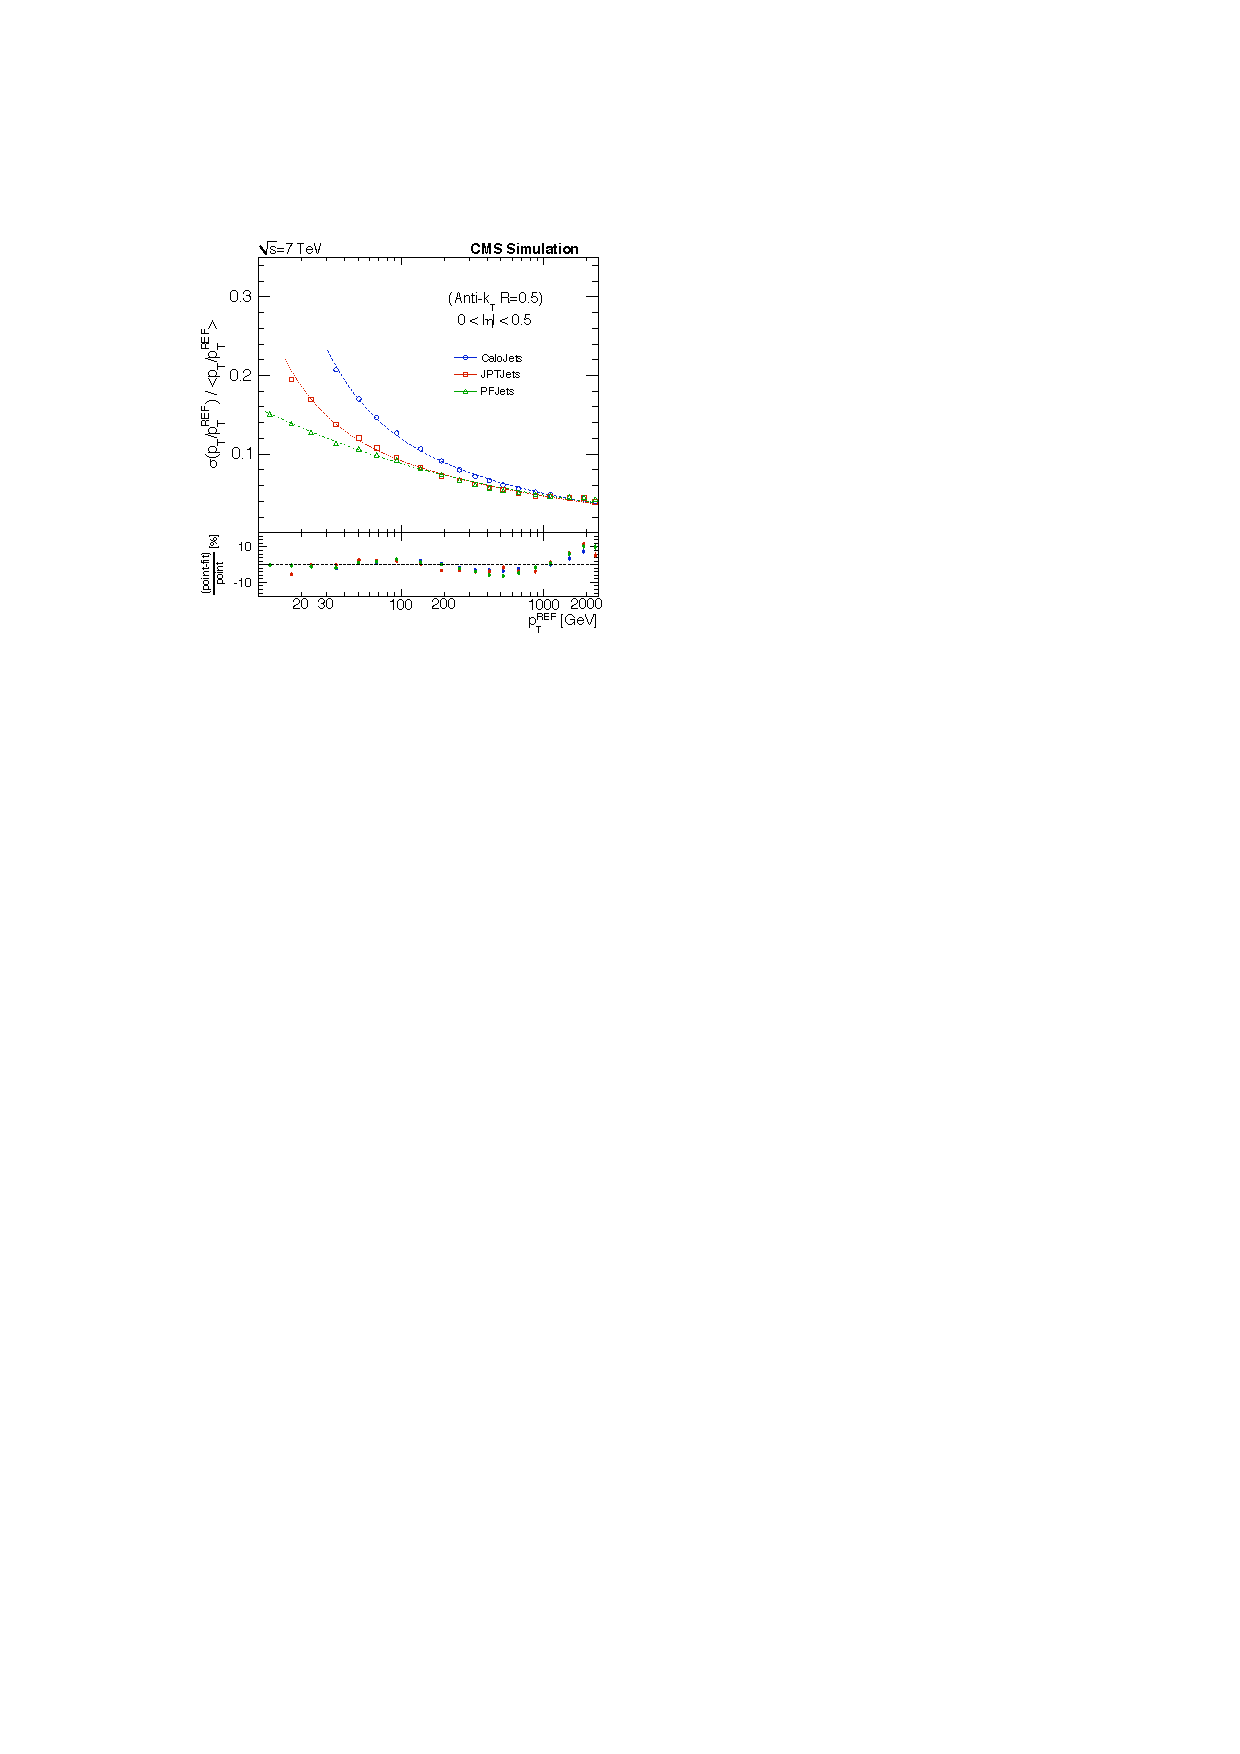
\includegraphics[width=0.5\textwidth]{jet_resolution.pdf}
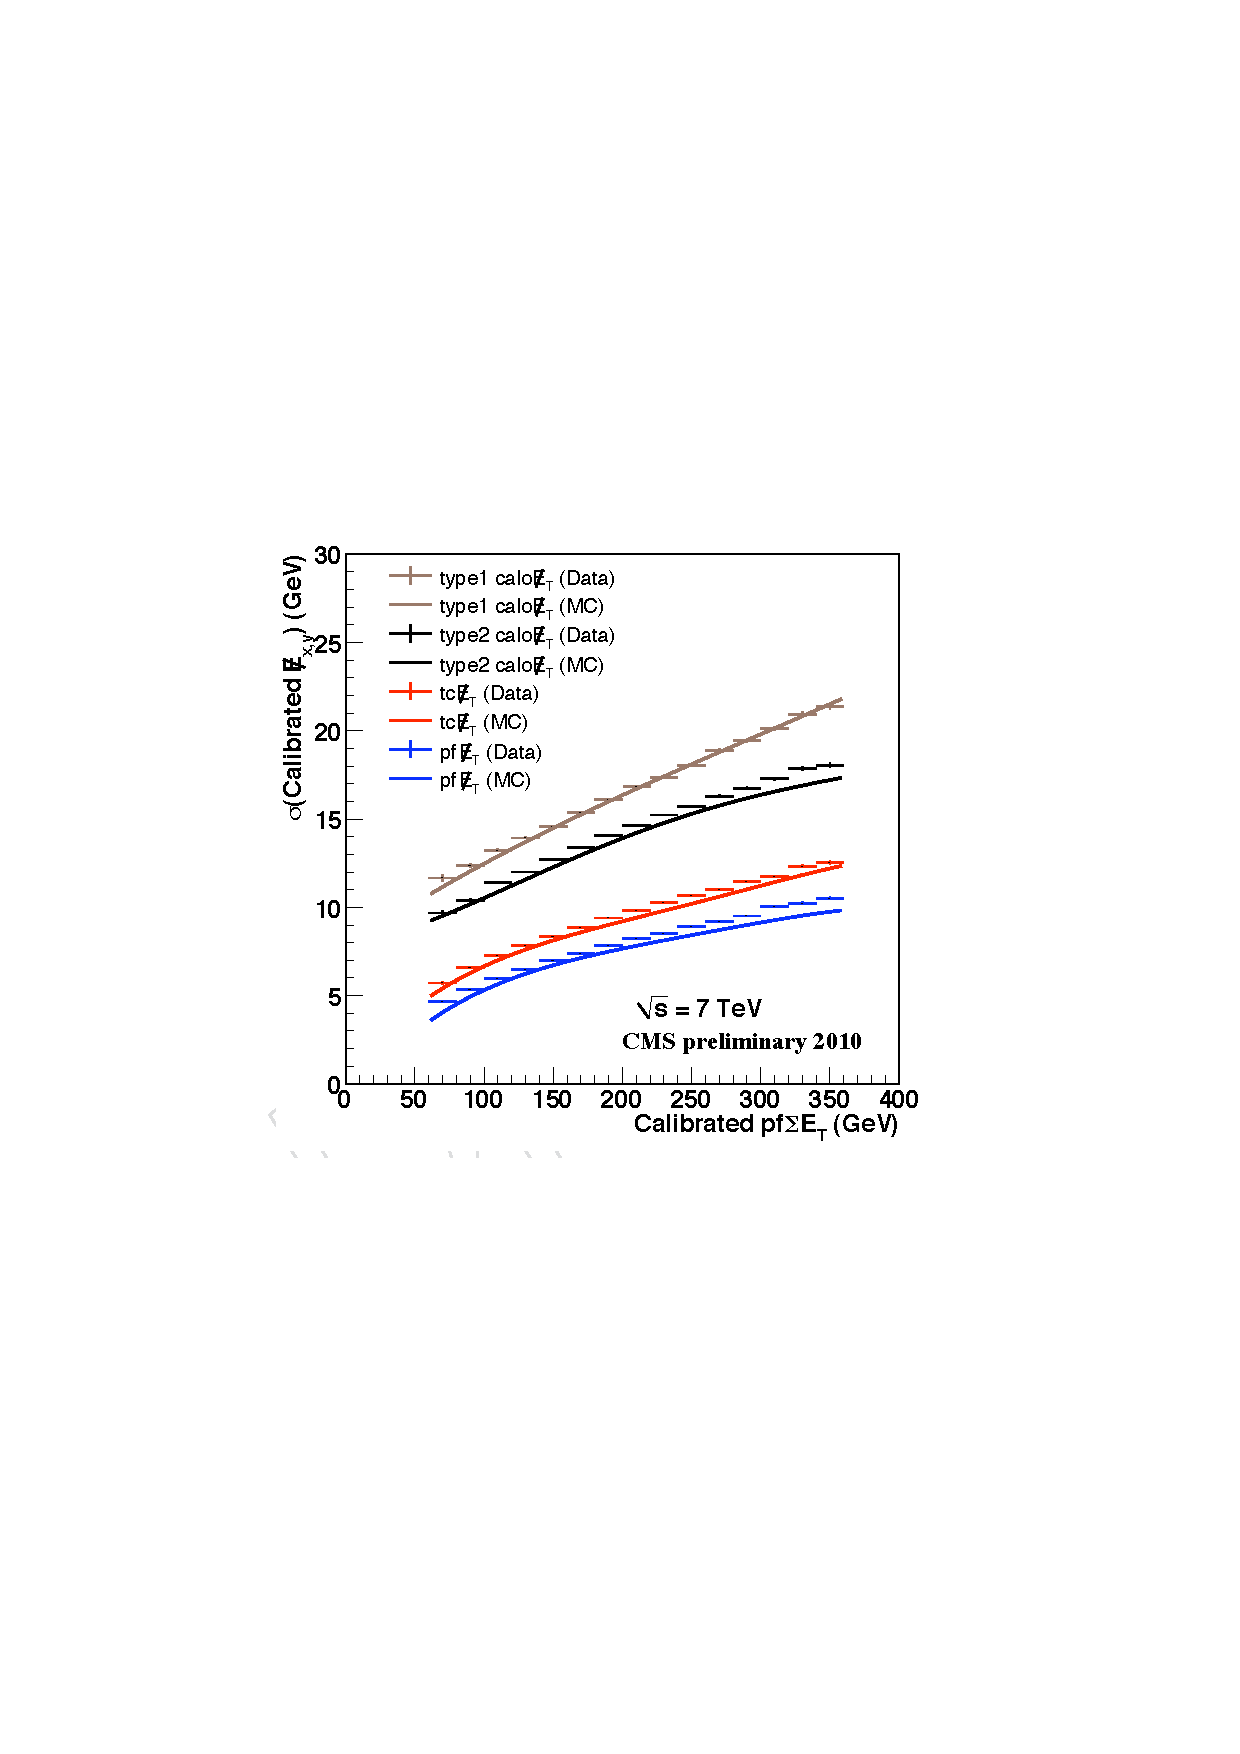
\includegraphics[width=0.5\textwidth]{met_resolution.pdf}
\caption{Performance measures for the HCAL: (a) the jet $\pT$ resolution as a 
function of jet $\pT$ for various different jet reconstructions and (b) the 
$\MET$ resolution as a function of Sum $\ET$ for different $\MET$
reconstructions. Reproduced from \cite{jet_resolution, met_resolution}.}
\label{fig:jetmet}
\end{figure}

\section{Superconducting Solenoid Magnet}

The superconducting solenoid generates a uniform 3.8T magnetic field. The 
magnetic field is important for determining the charge of particles and for the 
momentum measurement of charged particles, particularly low momentum charged 
particles and muons. The solenoid is 12.5m in length and 6m in diameter. The flux 
is returned through an iron yoke to provide a magnetic field which bends muons in 
the opposite direction. The iron is in layers between the muon chambers. \\

The precision of the momentum measurements in the inner tracker relies on a
homogeneous magnetic field. Within the tracker the magnetic field is homogeneous
to within 5\% \cite{field_measurement} and has been mapped with a precision 
better than 0.1\% \cite{field_uniformity}.

\section{Muon System}

The purpose of the muon system is the identification and triggering of muons. It
also provides a momentum measurement of the muons. \\

The muon system has a barrel region in the pseudorapidity range $\eta < 1.2$ and
two endcaps with $1.2 < \eta < 2.4$. Standard drift tube chambers are used in
the barrel and cathode strip chambers in the endcaps. The muon ionises the gas 
as it passes through the chamber. The resolution increases with the $\pT$ of the
muon since the straighter the track the more difficult it is to accurately 
determine the curvature. Also the resolution is worse in the endcaps where the
fake rate is higher and the magnetic field is less uniform. Figure
\ref{fig:muon_resolution} shows the muon $\pT$ resolution as a function of muon
$\pT$.

\begin{figure}
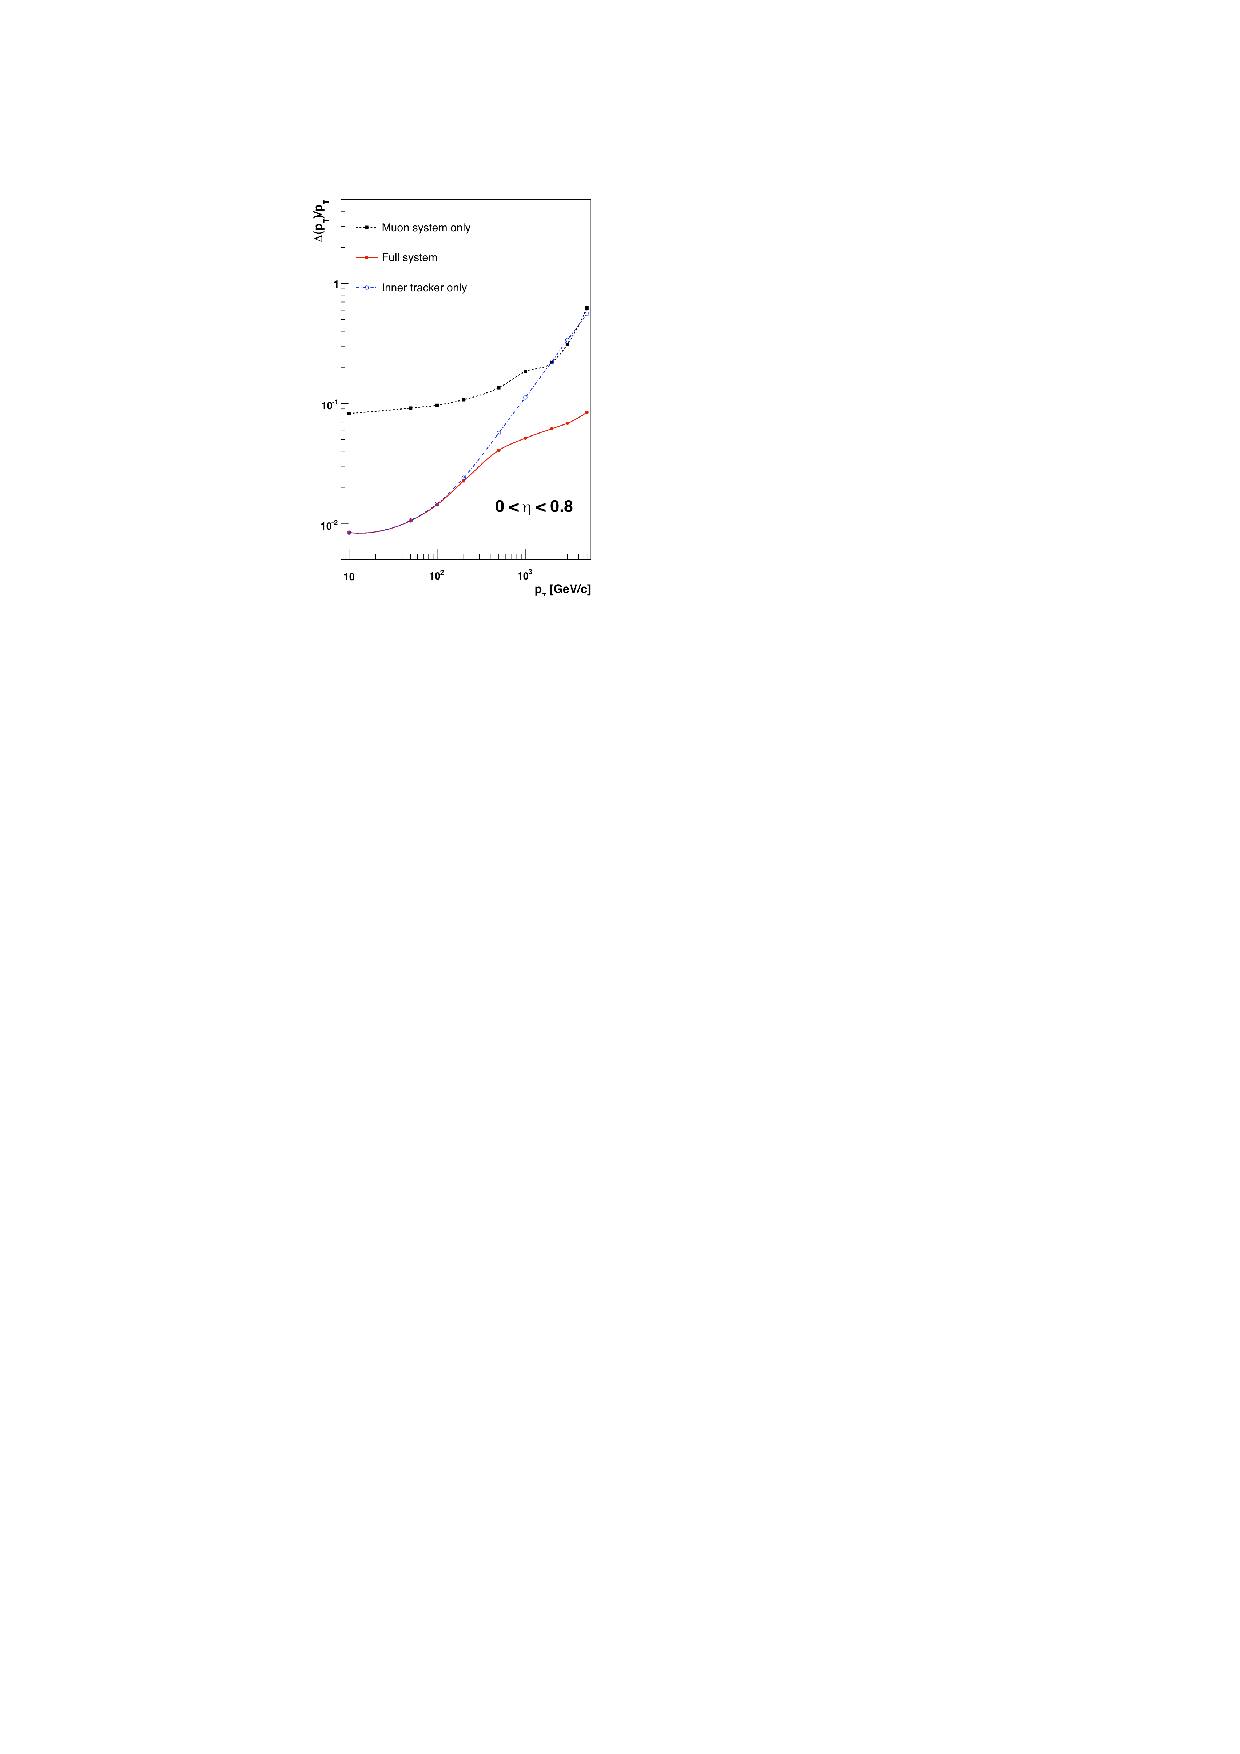
\includegraphics[width=0.5\textwidth]{muon_res_barrel.pdf}
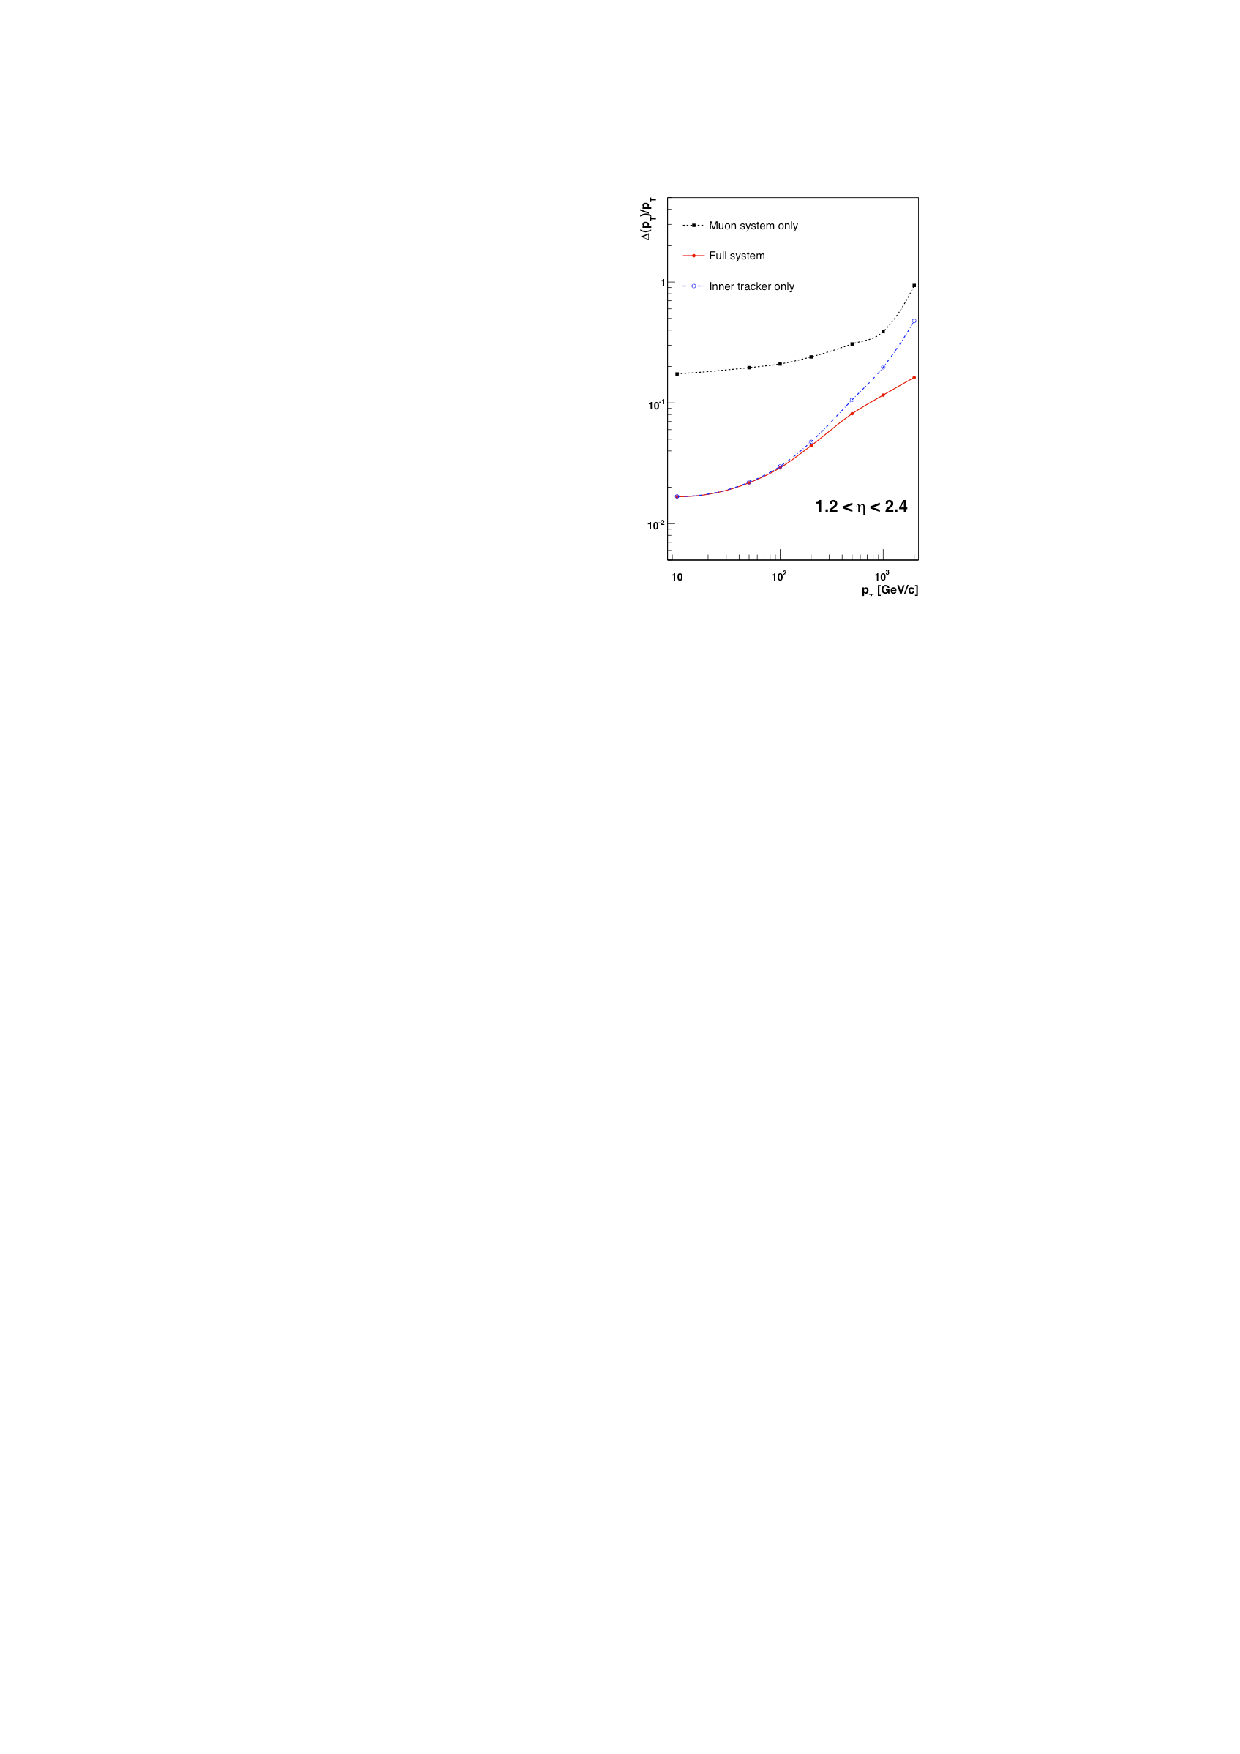
\includegraphics[width=0.5\textwidth]{muon_res_endcap.pdf}
\caption{The muon $\pT$ resolution as a function of muon $\pT$ for (a) $\eta <
0.8$ and (b) $1.2 < \eta < 2.4$. Reproduced from \cite{muon_resolution}.}
\label{fig:muon_resolution}
\end{figure}

\section{Trigger}

With a soft QCD cross-section of $\sim1\unit{mb}$ and a luminosity of
$10^{33}\unit{cm^{-1}s^{-1}}$ 
%($1\unit{nb^{-1}s^{-1}$) 
the event rate is $\sim 1
\unit{MHz}$. However, most of these are uninteresting soft QCD events. Intresting events such
as W/Z production, Higgs production or SUSY events have much smaller 
cross-sections. Figure \ref{fig:cross_sections} shows the cross sections of
various processes. Also there is a technical limit on the rate at which data can
be read out. The CMS data acquisition (DAQ) bandwidth limits the event rate to 
$\sim 100\unit{kHz}$. Offline reconstruction and storage facilities further limit the
rate to $\sim 100\unit{Hz}$. The goal of the trigger is to select the interesting 
events to read out and process. \\

\begin{figure}
\begin{center}
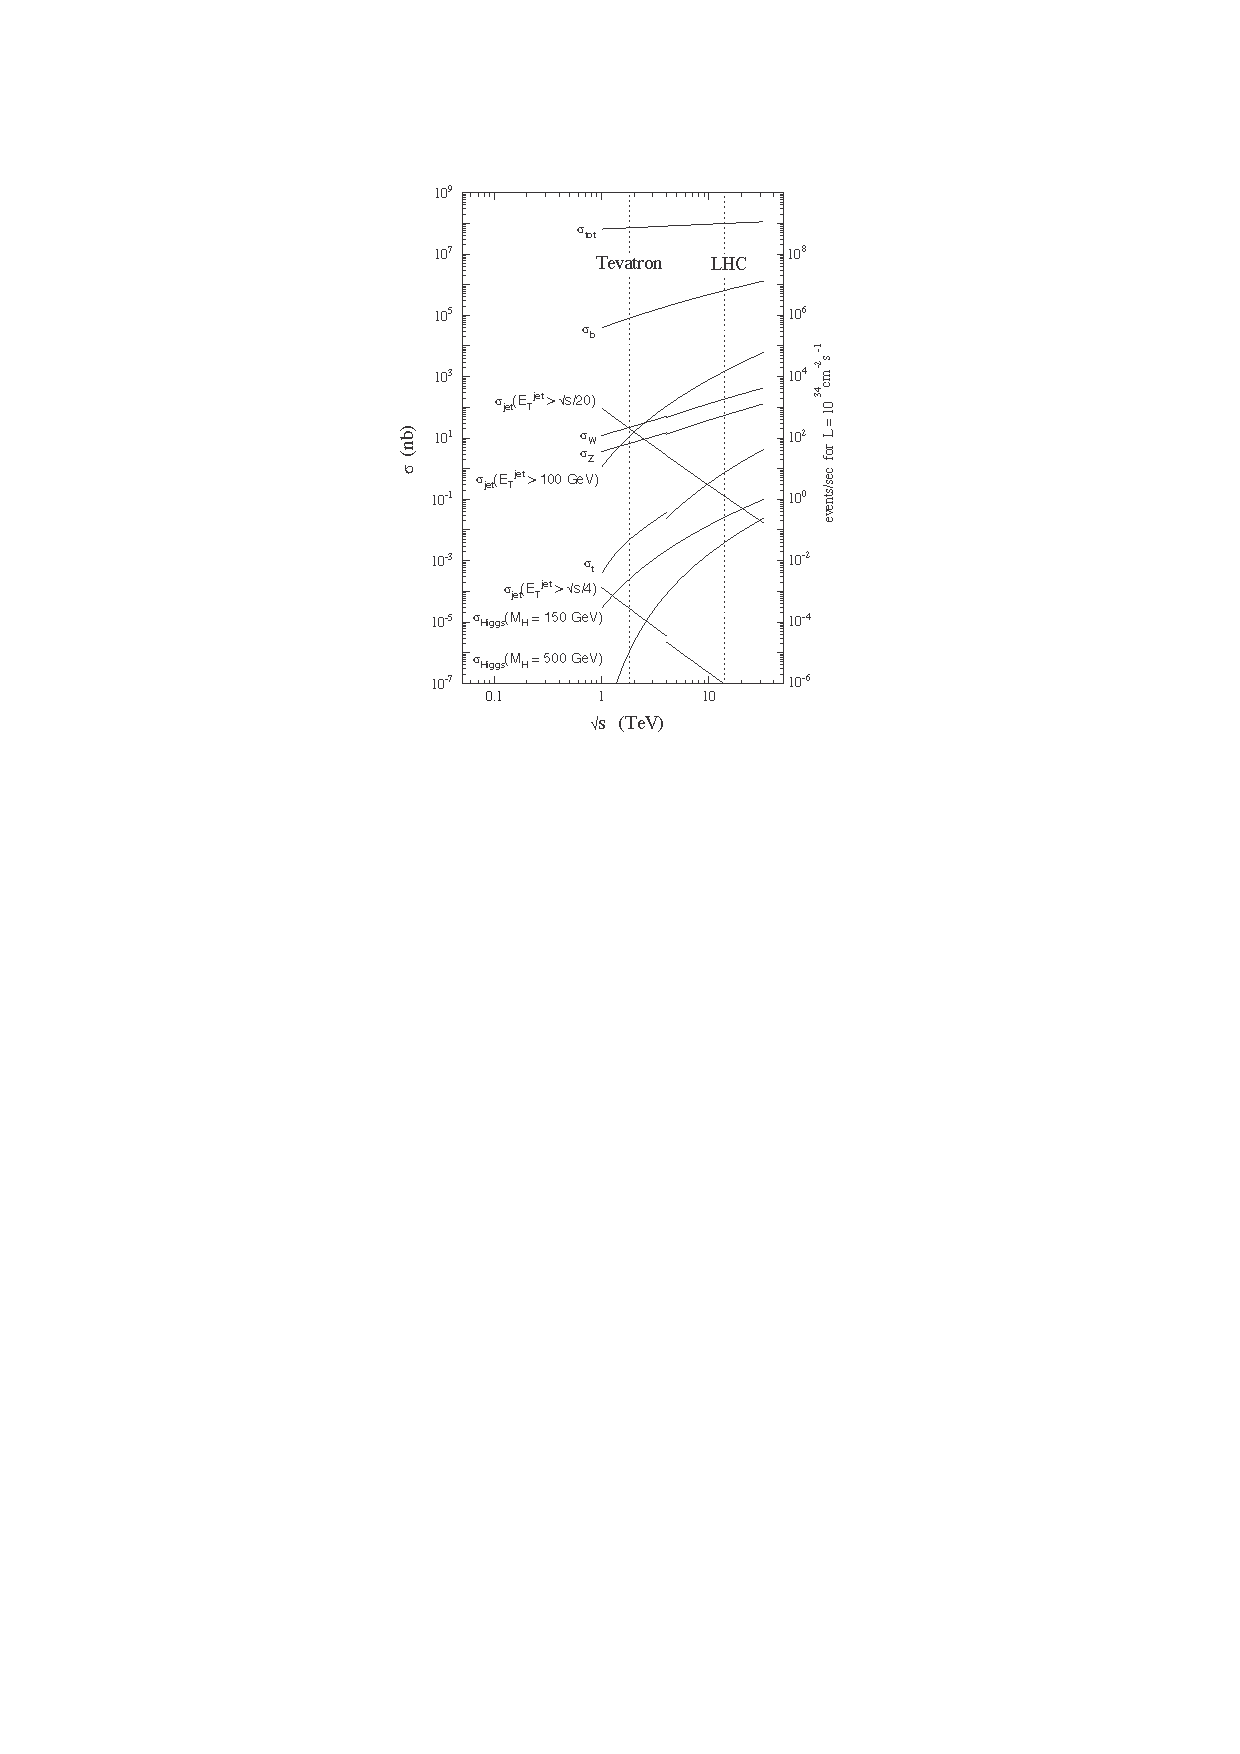
\includegraphics[width=0.7\textwidth]{Cross_Sections.pdf}
\end{center}
\caption{The cross-sections of various processes as a function of centre-of-mass
energy.}
\label{fig:cross_sections}
\end{figure}

There are two components to the trigger: Level 1 and HLT. Level 1 consists of
on-detector hardware and the goal is to reduce the rate to $\sim 10\unit{kHz}$ to
satisfy the constraint set by the DAQ bandwidth. The HLT is run on a farm of 
computers in a room above the CMS detector. It reconstructs physics objects 
and makes decisions based on the presence and quality of these to further reduce
the rate to $\sim 100\unit{Hz}$ to satisfy the constraint set by the storage and 
reconstruction facilities.

\section{CMS Computing Model}

CMS has produced O(100PB) of data and the quantity is growing. No single computer
centre is capable of handling such a large quantity of data. The CMS computing
model involves a network of data centres across the world (Figure 
\ref{fig:CMS_Data_Centres}) in a hierarchy of Tiers. 

\begin{itemize}
\item Tier 0 is the data centre at CERN which is directly connected to the
experiment. It stores the RAW data and produces the first reconstruction which
is subsequently transferred to Tier 1 sites. 
\item Data from Tier 0 is distributed to 8 Tier 1 sites. Each Tier 1 site is 
responsible for storing a second copy of the RAW and reconstructed data. A lot 
of reprocessed data is also stored at the Tier 1 sites. 
\item Data from the Tier 1 sites is transferred to 38 Tier 2 sites. These data
centres store data for analysis by CMS physicists. Data at the Tier 2 sites is
not complete and is not stored permanently, but is updated based on the
requirements of the CMS collaboration. 
\end{itemize}

\begin{figure}
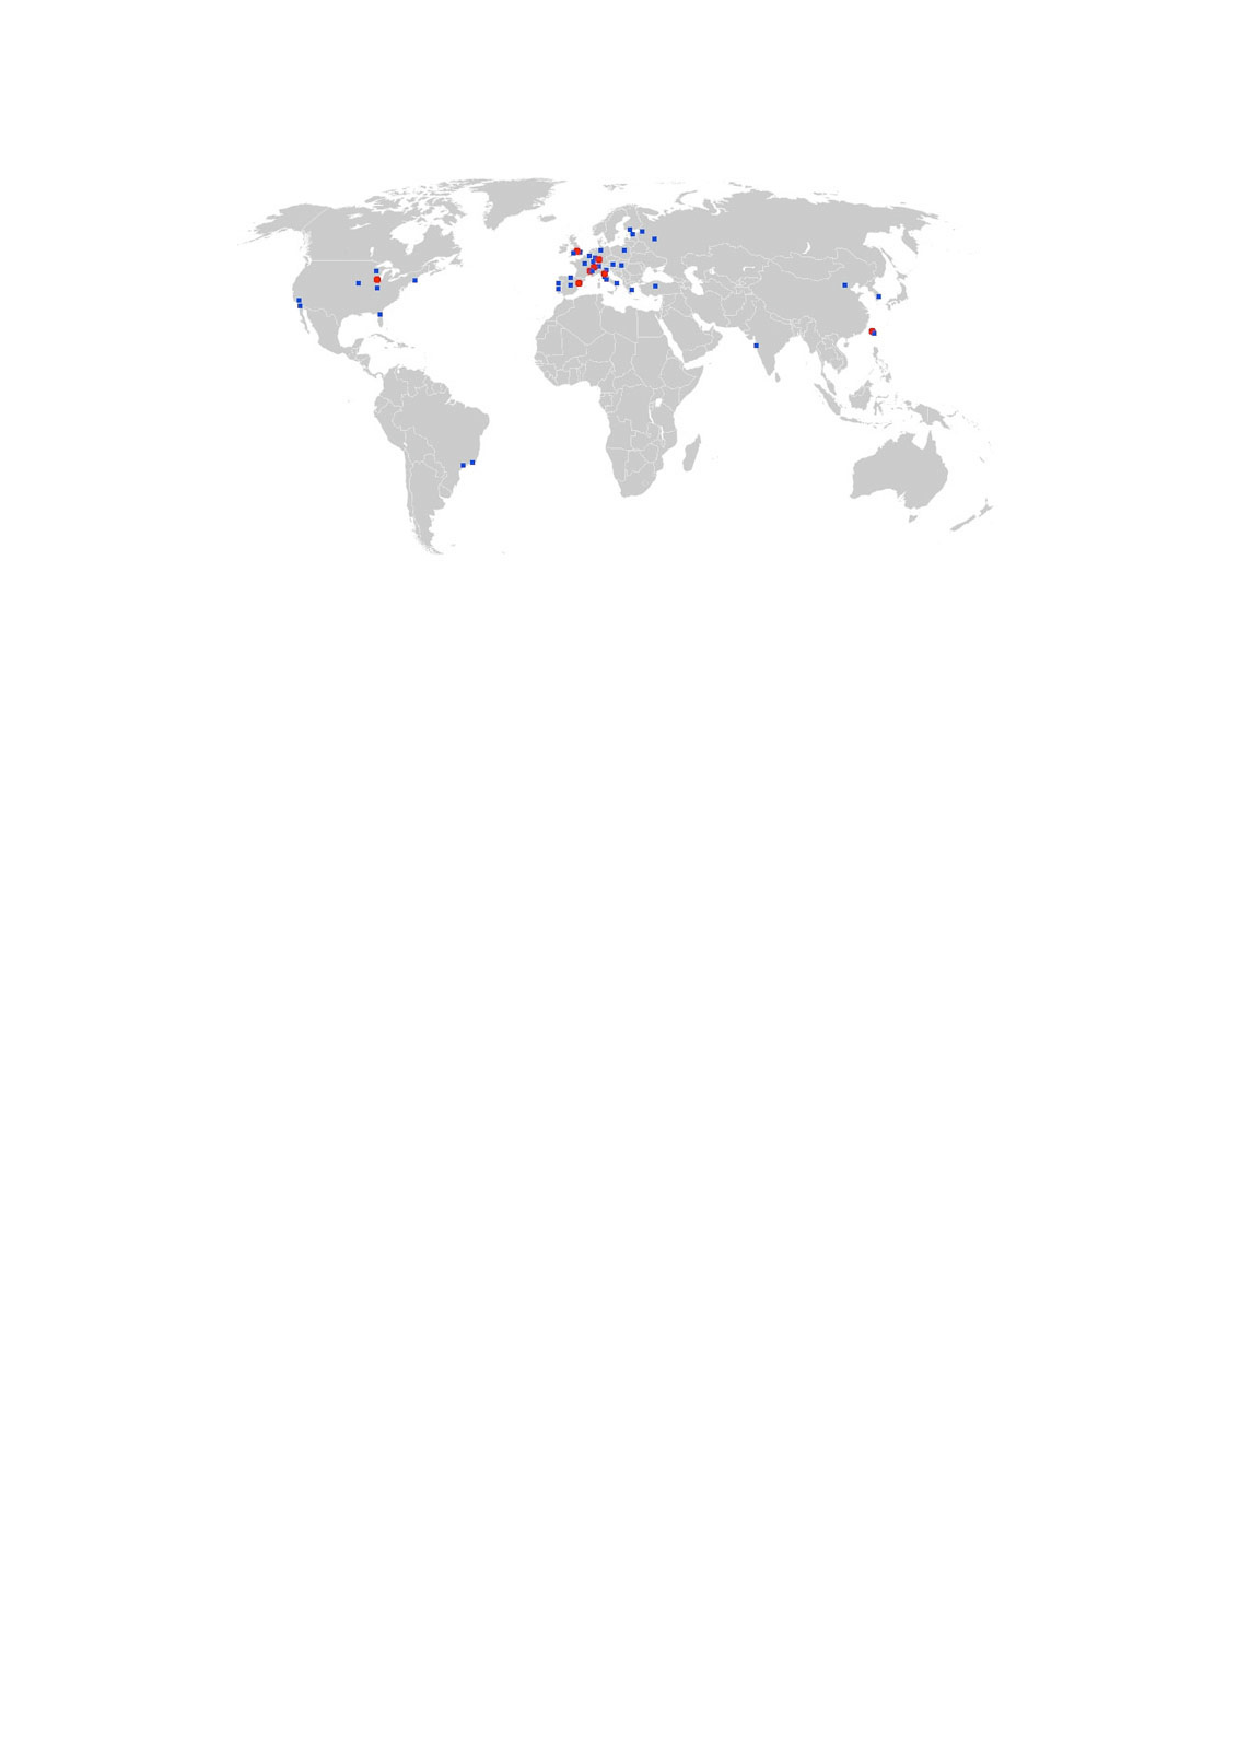
\includegraphics[width=\textwidth]{CMS_Data_Centres.pdf}
\caption{A map showing the geographical distribution of CMS Tier 1 (red dots)
and Tier 2 (blue dots) data centres. Reproduced from \cite{grid}.}
\label{fig:CMS_Data_Centres}
\end{figure}

\section{Photon Reconstruction}
\label{sec:photon_recontruction}

Photons make electromagnetic showers in the ECAL. Electromagnetic showers are 
reconstructed from the energy deposits in the ECAL crystals. The clustering 
algorithm starts with the energy deposits in single crystals and groups these 
together starting with the highest energy crystal. A strip 5 crystals wide in 
the $\eta$ direction and with dynamic $\phi$ length is used to contain the 
energy in the cluster or clusters. To incorporate bremstrahlung from electrons, 
the strip can be extended in the $\phi$ direction. A description of the
superclustering algorithm is given here \cite{supercluster}. \\ 

Fake photons from QCD come from jets and so tend to have plenty of activity in
the surrounding detectors. In contrast, prompt photons tend to be isolated with
little surrounding activity. Isolation is one of the variables used to select 
photons because of its background rejection power. There are three independent 
isolation measures based on the ECAL, the HCAL and the tracker. \\

Fake photons from jets also tend to have a hadronic component as well as an
electromagnetic component while prompt photons are purely electromagnetic.
Electromagnetic showers have a particular shower shape. Prompt photons can be 
distinguished from fakes by the shower shape. Photons are distinguished from 
electrons by the tracker. Electrons, being charged particles, ionise in the 
silicon tracker and so leave a track. Photons do not. \\ 

Based on these considerations, there are six variables used for the photon 
selection:

\begin{itemize}
\item {\bf ECAL isolation} is defined as the sum of the energy deposited in the
crystals of the ECAL in a $\Delta R = 0.4$ circle around the photon. A smaller 
circle of $\Delta R = 0.1$ around the photon is excluded from the isolation sum 
to avoid counting the photon itself in the isolation. Also a strip along $\phi$ 
of width $\Delta \eta = 0.04$ is excluded from the isolation sum to avoid 
including bremstrahlung from electrons. Figure \ref{fig:ECAL_Isolation} shows a
plot of the ECAL isolation of photon candidates for a SUSY model and the QCD 
background along with the cut value used in this analysis.

\begin{figure}
\begin{center}
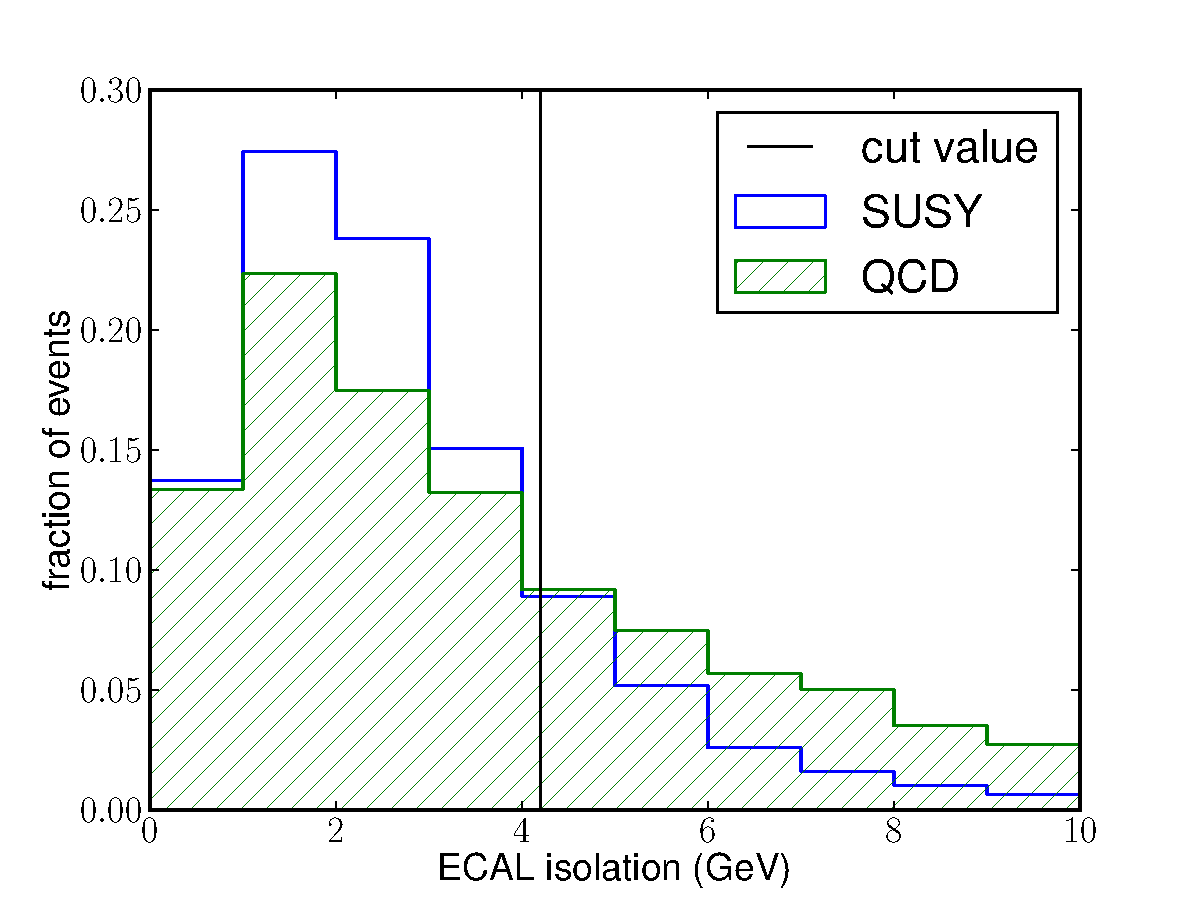
\includegraphics[width=0.8\textwidth]{ECAL_Isolation.pdf}
\end{center}
\caption{The ECAL isolation of photon candidates for a SUSY model and the QCD 
background along with the cut value used in this analysis.}
\label{fig:ECAL_Isolation}
\end{figure}

\item {\bf HCAL isolation} is defined as the sum of the energy deposited in the 
HCAL towers in a $\Delta R = 0.4$ circle around the photon position. A smaller 
circle of $\Delta R = 0.1$ is excluded from the isolation sum to avoid counting 
rear-leakage from high energy photons in the isolation. Figure 
\ref{fig:HCAL_Isolation} shows a plot of the HCAL isolation of photon candidates 
for a SUSY model and the QCD background along with the cut value used in this 
analysis.


\begin{figure}
\begin{center}
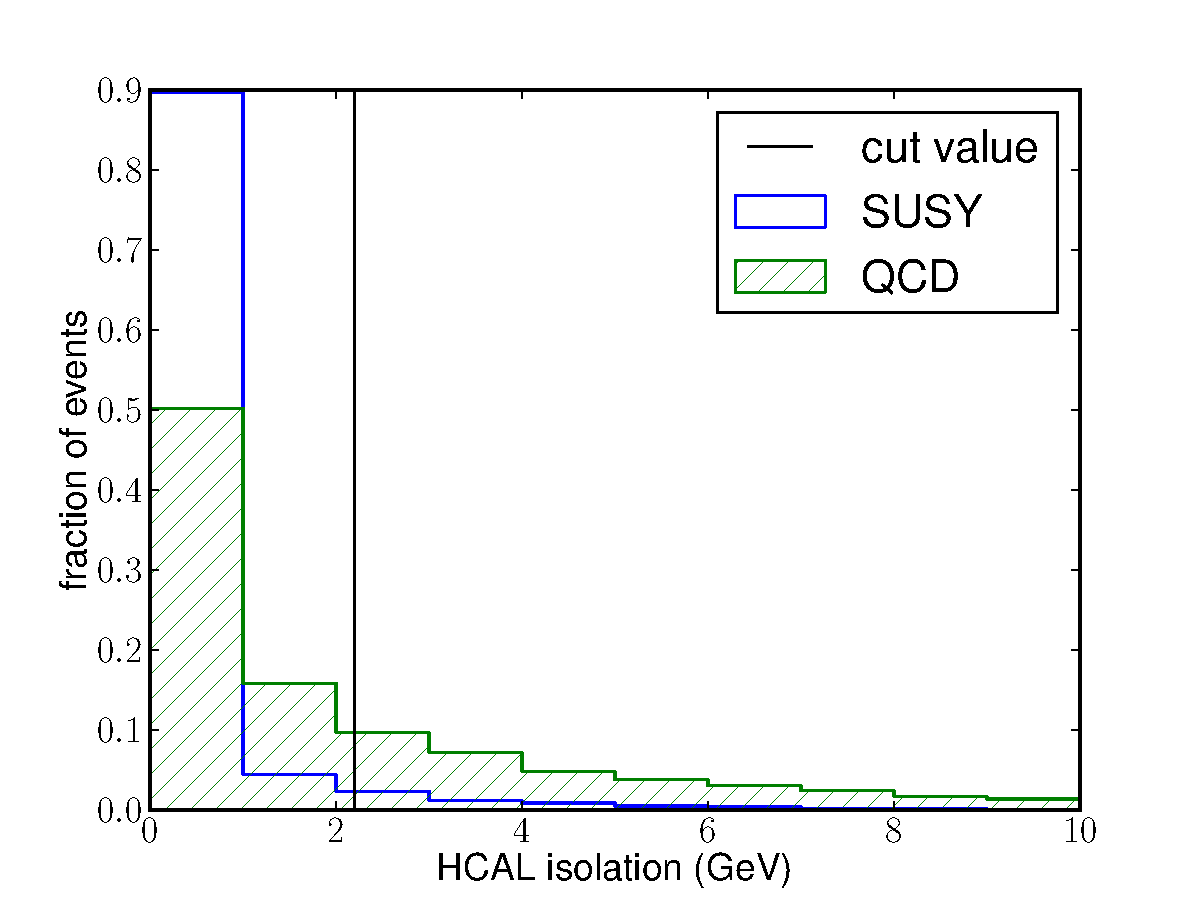
\includegraphics[width=0.8\textwidth]{HCAL_Isolation.pdf}
\end{center}
\caption{The HCAL isolation of photon candidates for a SUSY model and the QCD 
background along with the cut value used in this analysis.}
\label{fig:HCAL_Isolation}
\end{figure}

\item {\bf Track isolation} is defined as the sum of the $p_{T}$ of tracks 
inside a cone of $\Delta R = 0.4$ around the photon and toward the primary 
vertex. A hollow cone is used $\Delta R < 0.1$ is excluded from the isolation 
sum. Figure \ref{fig:Track_Isolation} shows a plot of the track isolation of
photon candidates for a SUSY model and the QCD background along with the cut 
value used in this analysis.


\begin{figure}
\begin{center}
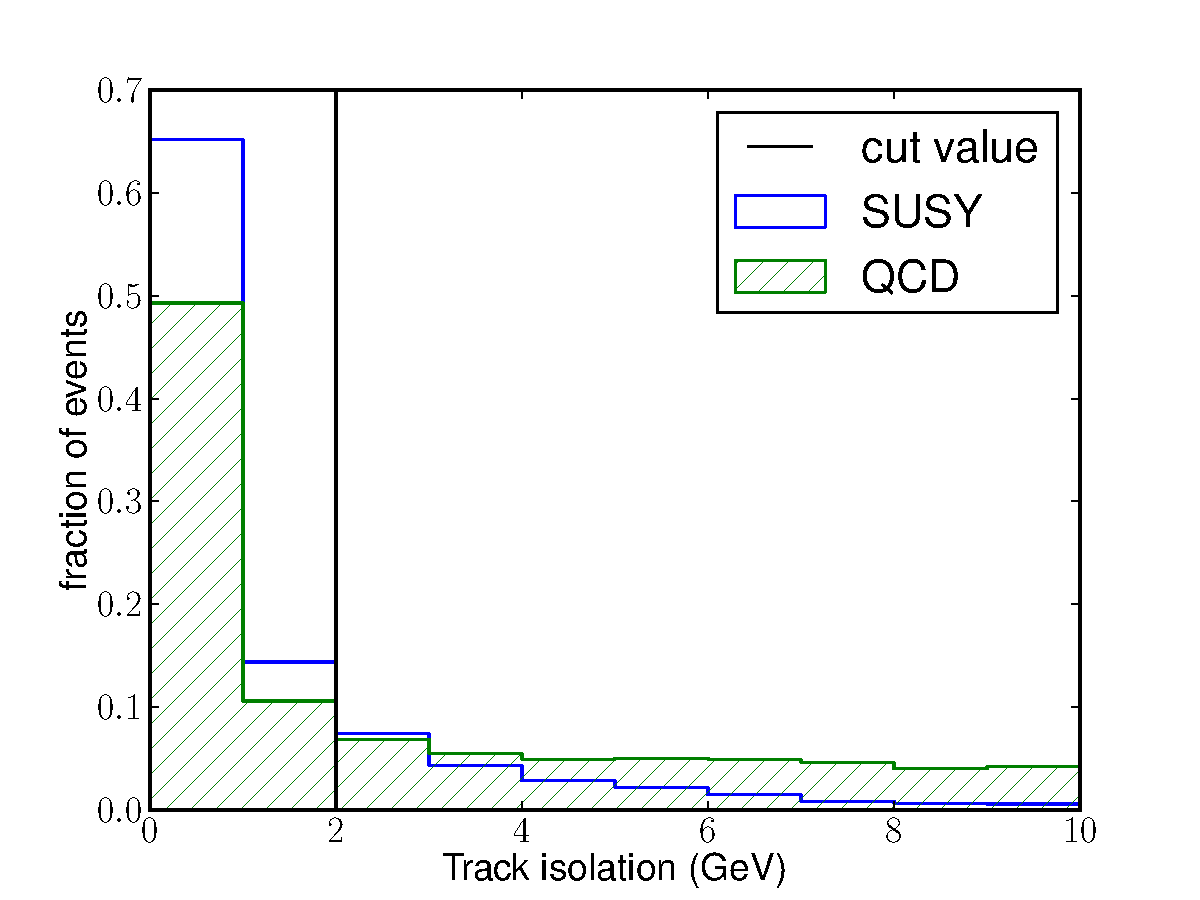
\includegraphics[width=0.8\textwidth]{Track_Isolation.pdf}
\end{center}
\caption{The track isolation of photon candidates for a SUSY model and the QCD 
background along with the cut value used in this analysis.}
\label{fig:Track_Isolation}
\end{figure}

\item {\bf H/E} is the ratio of the hadronic energy deposited in the HCAL behind
the photon to the photon energy. Jets faking photons are likely to have a 
significant amount of hadronic energy while for prompt photons the amount of 
hadronic energy is likely to be small. Figure \ref{fig:Hadronic_Over_EM} shows a
plot of the H/E of photon candidates for a SUSY model and the QCD background 
along with the cut value used in this analysis.

\begin{figure}
\begin{center}
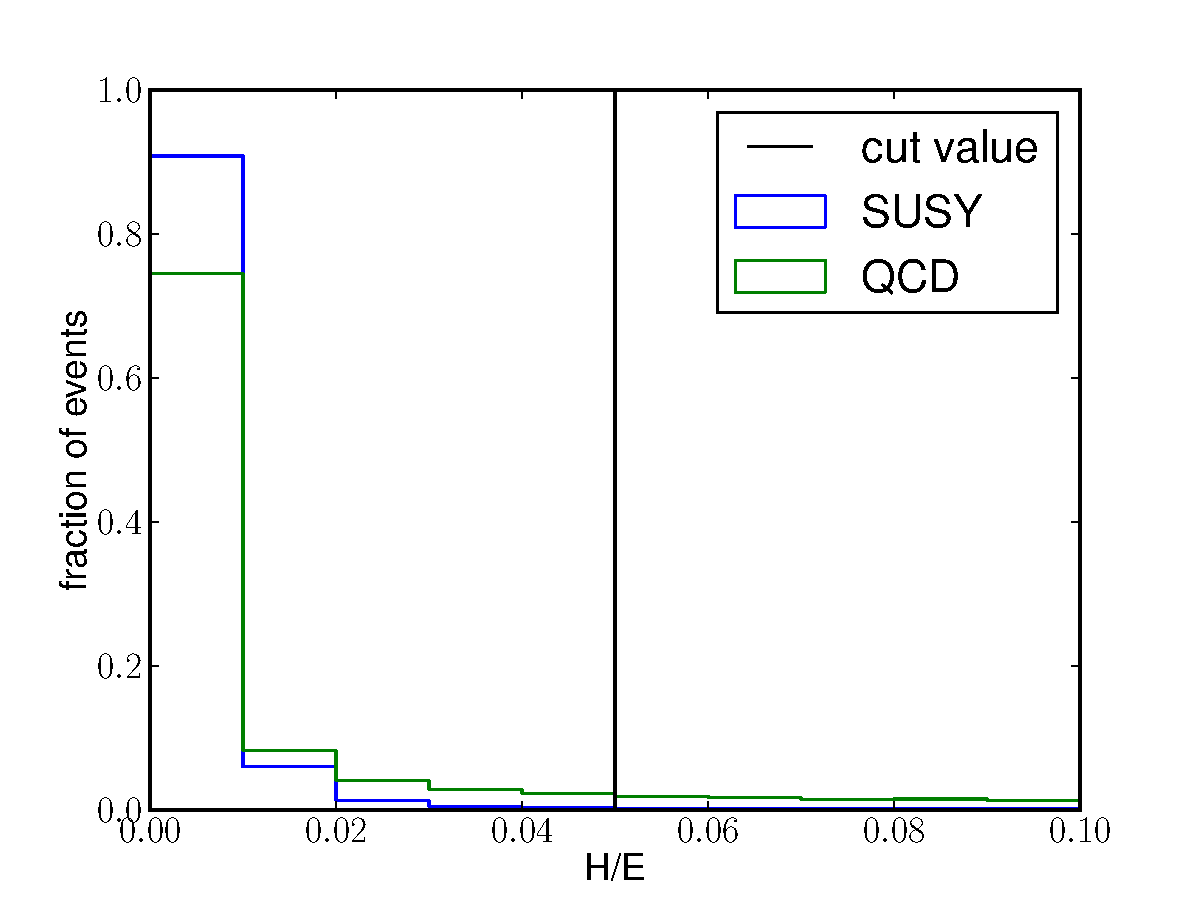
\includegraphics[width=0.8\textwidth]{Hadronic_Over_EM.pdf}
\end{center}
\caption{The H/E of photon candidates for a SUSY model and the QCD background 
along with the cut value used in this analysis.}
\label{fig:Hadronic_Over_EM}
\end{figure}

\item {\bf Shower Shape ($\sigma_{i\eta i\eta}$)}. The width of the shower in 
the $\eta$ direction is used as a measure of the shower shape. The $\eta$ 
direction rather than the $\phi$ direction is used because bremstrahlung can 
cause electromagnetic showers to be spread out in $\phi$. $\sigma_{\eta\eta}$ is
the r.m.s width of the shower in the $\eta$ direction. The variable used here is
$\sigma_{i\eta i\eta}$, which calculates the width in terms of number of 
crystals in the $\eta$ direction rather than $\eta$ itself. This is better 
because it does not count the gaps between crystals (where there is no 
showering) in the width and it is not distorted by the geometry of the detector 
in the end-cap region. Figures \ref{fig:SigmaIetaIeta_EB} and
\ref{fig:SigmaIetaIeta_EE} show plots of the shower shape of photon candidates 
in the ECAL barrel and ECAL end-cap respectively. The distributions are shown 
for a SUSY model and the QCD background along with the cut value used in this 
analysis.

\begin{figure}
\begin{center}
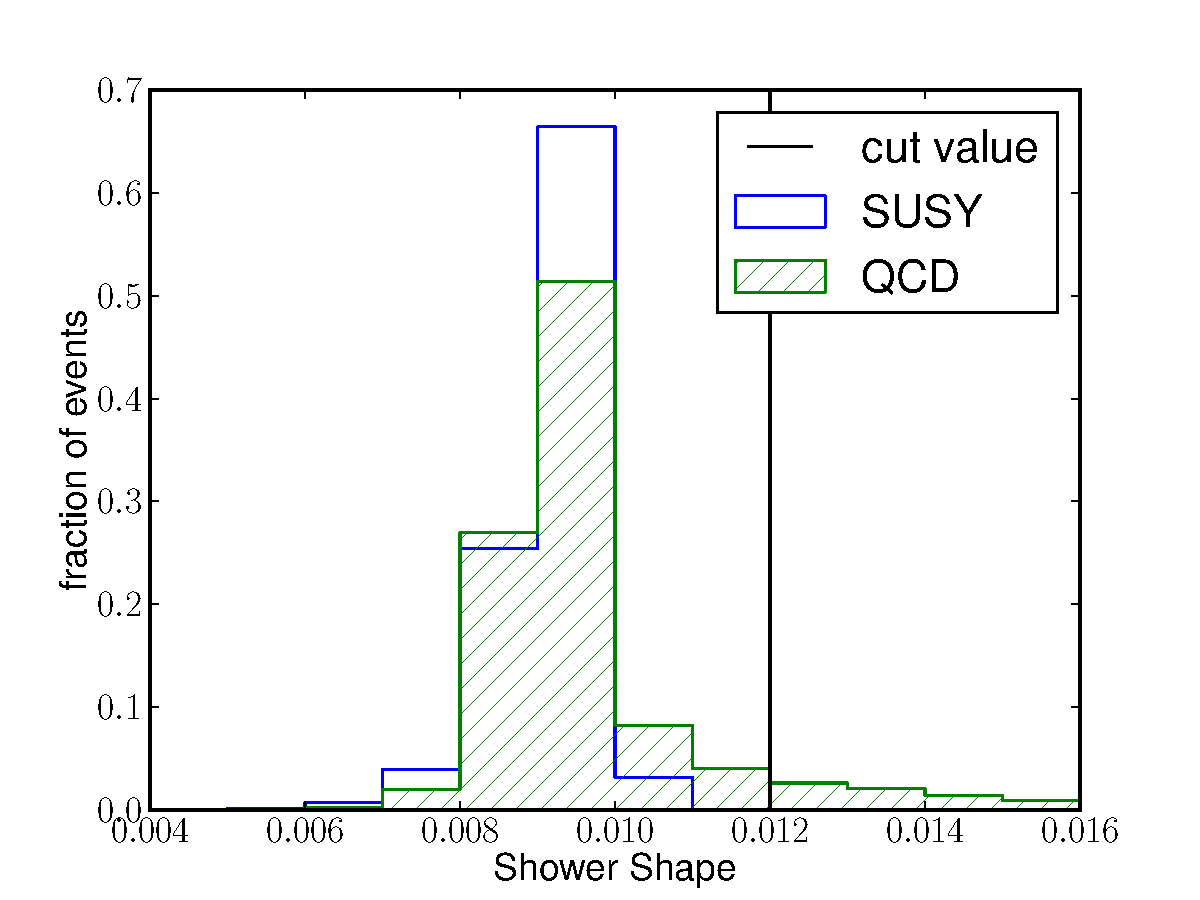
\includegraphics[width=0.8\textwidth]{SigmaIetaIeta_EB.pdf}
\end{center}
\caption{The shower shape of photon candidates in the ECAL barrel for a SUSY 
model and the QCD background along with the cut value used in this analysis.} 
\label{fig:SigmaIetaIeta_EB}
\end{figure}

\begin{figure}
\begin{center}
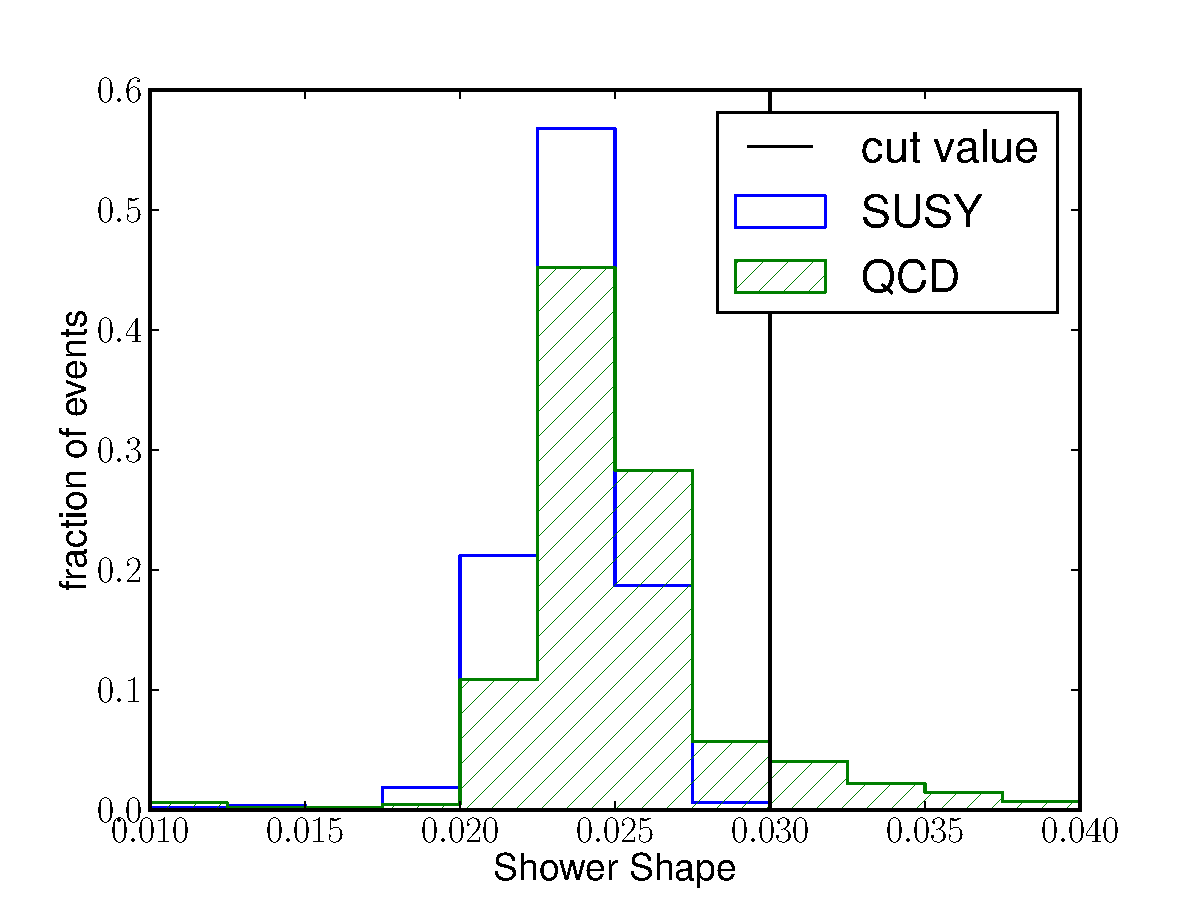
\includegraphics[width=0.8\textwidth]{SigmaIetaIeta_EE.pdf}
\end{center}
\caption{The shower shape of photon candidates in the ECAL end-cap for a SUSY 
model and the QCD background along with the cut value used in this analysis.} 
\label{fig:SigmaIetaIeta_EE}
\end{figure}

\item {\bf Pixel Seed}. A pixel seed is a track stub in the pixel detector that 
is the first step in track reconstruction. The photon selection requires that 
there is no pixel seed corresponding to the electromagnetic shower.
\end{itemize}

\section{Jet Reconstruction}

Jets are collimated bunches of stable hadrons originating from partons (quarks
and gluons) after fragmentation and hadronisation. Jets are reconstructed based 
on energy deposits in the detector using the Anti-KT jet algorithm with a cone 
size of $\Delta R = 0.5$. The Anti-KT jet algorithm is a clustering, cone 
algorithm which does not suffer from the problem of infra red and collinear 
divergences. \\

Under the anti-KT algorithm energy deposits are clustered together within a cone
according to their distance from each other. The ``distance'', $d_{ij}$, between 
objects (energy deposits/particles) is defined by Equation \ref{eq:distance}.

\begin{equation}
d_{ij} = min(p_{T1}^{-2}, p_{T2}^{-2})\frac{\Delta_{ij}}{R}
\label{eq:distance}
\end{equation}

$\Delta_{ij} = \sqrt{\Delta \eta^{2} + \Delta \phi^{2}}$ and R is the radius of
the cone. \\

The Anti-KT algorithm is the most widely used within CMS because it has higher 
efficiency than the other algorithms (ref). Figure.
